% Options for packages loaded elsewhere
% Options for packages loaded elsewhere
\PassOptionsToPackage{unicode}{hyperref}
\PassOptionsToPackage{hyphens}{url}
\PassOptionsToPackage{dvipsnames,svgnames,x11names}{xcolor}
%
\documentclass[
  spanish]{cyta}
\usepackage{xcolor}
\usepackage{amsmath,amssymb}
\setcounter{secnumdepth}{-\maxdimen} % remove section numbering
\usepackage{iftex}
\ifPDFTeX
  \usepackage[T1]{fontenc}
  \usepackage[utf8]{inputenc}
  \usepackage{textcomp} % provide euro and other symbols
\else % if luatex or xetex
  \usepackage{unicode-math} % this also loads fontspec
  \defaultfontfeatures{Scale=MatchLowercase}
  \defaultfontfeatures[\rmfamily]{Ligatures=TeX,Scale=1}
\fi
\usepackage{lmodern}
\ifPDFTeX\else
  % xetex/luatex font selection
\fi
% Use upquote if available, for straight quotes in verbatim environments
\IfFileExists{upquote.sty}{\usepackage{upquote}}{}
\IfFileExists{microtype.sty}{% use microtype if available
  \usepackage[]{microtype}
  \UseMicrotypeSet[protrusion]{basicmath} % disable protrusion for tt fonts
}{}
\makeatletter
\@ifundefined{KOMAClassName}{% if non-KOMA class
  \IfFileExists{parskip.sty}{%
    \usepackage{parskip}
  }{% else
    \setlength{\parindent}{0pt}
    \setlength{\parskip}{6pt plus 2pt minus 1pt}}
}{% if KOMA class
  \KOMAoptions{parskip=half}}
\makeatother
% Make \paragraph and \subparagraph free-standing
\makeatletter
\ifx\paragraph\undefined\else
  \let\oldparagraph\paragraph
  \renewcommand{\paragraph}{
    \@ifstar
      \xxxParagraphStar
      \xxxParagraphNoStar
  }
  \newcommand{\xxxParagraphStar}[1]{\oldparagraph*{#1}\mbox{}}
  \newcommand{\xxxParagraphNoStar}[1]{\oldparagraph{#1}\mbox{}}
\fi
\ifx\subparagraph\undefined\else
  \let\oldsubparagraph\subparagraph
  \renewcommand{\subparagraph}{
    \@ifstar
      \xxxSubParagraphStar
      \xxxSubParagraphNoStar
  }
  \newcommand{\xxxSubParagraphStar}[1]{\oldsubparagraph*{#1}\mbox{}}
  \newcommand{\xxxSubParagraphNoStar}[1]{\oldsubparagraph{#1}\mbox{}}
\fi
\makeatother


\usepackage{longtable,booktabs,array}
\usepackage{calc} % for calculating minipage widths
% Correct order of tables after \paragraph or \subparagraph
\usepackage{etoolbox}
\makeatletter
\patchcmd\longtable{\par}{\if@noskipsec\mbox{}\fi\par}{}{}
\makeatother
% Allow footnotes in longtable head/foot
\IfFileExists{footnotehyper.sty}{\usepackage{footnotehyper}}{\usepackage{footnote}}
\makesavenoteenv{longtable}
\usepackage{graphicx}
\makeatletter
\newsavebox\pandoc@box
\newcommand*\pandocbounded[1]{% scales image to fit in text height/width
  \sbox\pandoc@box{#1}%
  \Gscale@div\@tempa{\textheight}{\dimexpr\ht\pandoc@box+\dp\pandoc@box\relax}%
  \Gscale@div\@tempb{\linewidth}{\wd\pandoc@box}%
  \ifdim\@tempb\p@<\@tempa\p@\let\@tempa\@tempb\fi% select the smaller of both
  \ifdim\@tempa\p@<\p@\scalebox{\@tempa}{\usebox\pandoc@box}%
  \else\usebox{\pandoc@box}%
  \fi%
}
% Set default figure placement to htbp
\def\fps@figure{htbp}
\makeatother





\setlength{\emergencystretch}{3em} % prevent overfull lines

\providecommand{\tightlist}{%
  \setlength{\itemsep}{0pt}\setlength{\parskip}{0pt}}



 
\usepackage[]{natbib}
\bibliographystyle{plainnat}


\usepackage{fontspec}

\usepackage{multirow}

\usepackage{multicol}

\usepackage{colortbl}

\usepackage{ulem}

\usepackage{hhline}

\newlength\Oldarrayrulewidth

\newlength\Oldtabcolsep

\usepackage{longtable}

\usepackage{array}

\usepackage{hyperref}

\usepackage{float}

\usepackage{wrapfig}

\PassOptionsToPackage{normalem}{ulem}
\usepackage{ulem}
\protected\def\emph#1{\textit{#1}}
\usepackage{float}
\makeatletter
\@ifpackageloaded{caption}{}{\usepackage{caption}}
\AtBeginDocument{%
\ifdefined\contentsname
  \renewcommand*\contentsname{Table of contents}
\else
  \newcommand\contentsname{Table of contents}
\fi
\ifdefined\listfigurename
  \renewcommand*\listfigurename{List of Figures}
\else
  \newcommand\listfigurename{List of Figures}
\fi
\ifdefined\listtablename
  \renewcommand*\listtablename{List of Tables}
\else
  \newcommand\listtablename{List of Tables}
\fi
\ifdefined\figurename
  \renewcommand*\figurename{Figure}
\else
  \newcommand\figurename{Figure}
\fi
\ifdefined\tablename
  \renewcommand*\tablename{Table}
\else
  \newcommand\tablename{Table}
\fi
}
\@ifpackageloaded{float}{}{\usepackage{float}}
\floatstyle{ruled}
\@ifundefined{c@chapter}{\newfloat{codelisting}{h}{lop}}{\newfloat{codelisting}{h}{lop}[chapter]}
\floatname{codelisting}{Listing}
\newcommand*\listoflistings{\listof{codelisting}{List of Listings}}
\makeatother
\makeatletter
\makeatother
\makeatletter
\@ifpackageloaded{caption}{}{\usepackage{caption}}
\@ifpackageloaded{subcaption}{}{\usepackage{subcaption}}
\makeatother
\usepackage{bookmark}
\IfFileExists{xurl.sty}{\usepackage{xurl}}{} % add URL line breaks if available
\urlstyle{same}
\hypersetup{
  pdftitle={De la Factoría Lineal a la Biorrefinería 4.0},
  colorlinks=true,
  linkcolor={blue},
  filecolor={Maroon},
  citecolor={Blue},
  urlcolor={Blue},
  pdfcreator={LaTeX via pandoc}}


\title{De la Factoría Lineal a la Biorrefinería 4.0}
\usepackage{etoolbox}
\makeatletter
\providecommand{\subtitle}[1]{% add subtitle to \maketitle
  \apptocmd{\@title}{\par {\large #1 \par}}{}{}
}
\makeatother
\subtitle{El salto de eficiencia técnica en el NOA}
\author{\normalsize \textbf{Marcelo Javier Lamarque}$^{1,2*}$, \textbf{Julio Rodríguez Rey}$^{2\dagger}$ y \textbf{Lorena Bearzotti}$^{3\ddagger}$ \\[0.4cm] \parbox{\textwidth}{\centering \footnotesize $^{1}$Facultad de Ingeniería, Universidad del Norte Santo Tomás de Aquino, Argentina.\\ $^{2}$CENIT - FACET, Universidad Nacional de Tucumán, Argentina.\\ $^{3}$Escuela de Ingeniería de Construcción y Transporte, Pontificia Universidad Católica de Valparaíso, Chile.} \\[0.4cm] \parbox{\textwidth}{\centering \scriptsize $^*$marcelo.lamarque@unsta.edu.ar \quad $^\dagger$jrodriguezrey@herrera.unt.edu.ar \quad $^\ddagger$lorena.bearzotti@pucv.cl}}
\date{2026-03-19}
\begin{document}
\maketitle
\begin{abstract}
\textbf{Resumen:} La industria azucarera del NOA enfrenta un agotamiento
del modelo productivo lineal. Este ensayo sostiene que la transición
hacia la Biorrefinería 4.0 es un imperativo de supervivencia
condicionado por la sofisticación analítica de las empresas. Se propone
un marco de hibridación donde el DEA-BCC orientado a outputs actúa como
diagnóstico de la eficiencia técnica (\(\theta\)) y algoritmos de Random
Forest operan como una ``autopsia digital'' para deconstruir el
\emph{Yield Gap}. Al analizar las 19 DMUs de la región con datos del
IPAAT, se demuestra que el cierre de la brecha operativa no depende solo
de la inversión física, sino de la capacidad de arbitrar flujos de
biomasa y energía mediante modelos prescriptivos que superen la
intuición analógica del pasado.

\textbf{Palabras clave:} Eficiencia Técnica; Biorrefinería 4.0; Análisis
Envolvente de Datos (DEA); Random Forest; Industria Azucarera del NOA;
Inteligencia Operativa; Analítica Prescriptiva.

\textbf{Abstract:} The sugar industry in Northwestern Argentina (NOA) is
facing the obsolescence of the linear production model. This essay
contends that the transition toward Biorefinery 4.0 is a survival
imperative, fundamentally conditioned by the firms' analytical
sophistication. A hybrid framework is proposed in which output-oriented
DEA-BCC serves as a diagnostic tool for technical efficiency
(\(\theta\)), while Random Forest algorithms function as a ``digital
autopsy'' to deconstruct the \emph{Yield Gap}. By analyzing the region's
19 DMUs using audited IPAAT data, it is demonstrated that closing the
operational gap depends not only on physical capital investment but also
on the strategic capacity to arbitrate biomass and energy flows through
prescriptive models that transcend the analog intuition of the past.

\textbf{Keywords:} Technical Efficiency; Biorefinery 4.0; Data
Envelopment Analysis (DEA); Random Forest; NOA Sugar Industry;
Operational Intelligence; Prescriptive Analytics.
\end{abstract}


\section{El Ocaso del Paradigma Azucarero
Tradicional}\label{el-ocaso-del-paradigma-azucarero-tradicional}

La industria azucarera del Noroeste Argentino (NOA) se encuentra en una
encrucijada histórica. El modelo del ingenio concebido exclusivamente
para la extracción de sacarosa ha quedado obsoleto ante las demandas de
la \textbf{economía circular} y la transición energética
\citep{dessbesell2017}.

La realidad operativa de Tucumán, Salta y Jujuy hoy se debate entre la
persistencia de una gestión intuitiva y la necesidad de una
transformación digital profunda. El problema no es solo la falta de
tecnología, sino la \textbf{brecha de madurez analítica}.

En el NOA, la toma de decisiones sigue anclada en análisis descriptivos
básicos (hojas de cálculo), lo que genera una ``ceguera operativa'' ante
las ineficiencias sistémicas. Como sostiene \citep{anino2018}, la
sostenibilidad del sector depende de su capacidad para mutar hacia
centros de valorización integral de biomasa.

\section{La Biorrefinería 4.0: Del ``Hardware'' a la Inteligencia
Operativa}\label{la-biorrefineruxeda-4.0-del-hardware-a-la-inteligencia-operativa}

La literatura académica clásica postula que la integración de una
destilería de bioetanol posee el potencial teórico de actuar como un
\textbf{catalizador termodinámico} \citep{bonomi2011}. En términos de
Investigación de Operaciones, la destilería se concibe como un
``amortiguador'' (\emph{buffer}) que permite expandir la frontera de
posibilidades de producción del ingenio, ofreciendo beneficios como:

\begin{itemize}
\tightlist
\item
  \textbf{Flexibilización del Output:} Desviar jugos de baja pureza
  hacia la producción de alcohol, optimizando el rendimiento global de
  la caña.
\item
  \textbf{Estabilidad Térmica:} Un mejor aprovechamiento del bagazo y el
  vapor, transformando el excedente energético en productos de alto
  valor.
\end{itemize}

Sin embargo, desde una perspectiva de consultoría estratégica y
analítica avanzada, este ensayo argumenta que \textbf{el simple
emplazamiento de una planta de bioetanol (el ``hardware'' industrial) no
garantiza el salto hacia la frontera de eficiencia}.

La evidencia demuestra que los ingenios tradicionales operan bajo una
lógica lineal donde la destilería suele ser tratada como un silo anexo y
no como un sistema integrado. Para que la teórica flexibilidad de la
Biorrefinería se traduzca en una eficiencia técnica (\(\theta\)) real y
resiliente frente a la variabilidad de la materia prima
\citep{bogetoft2011}, se requiere una transición hacia la
\textbf{Biorrefinería 4.0} \citep{pessl2017, ghobakhloo2018}.

Esto implica abandonar la gestión intuitiva para adoptar una
\textbf{Inteligencia Operativa basada en datos} \citep{petrus2024},
donde el volumen procesado (Escala) y la asignación dinámica de flujos
(Diversificación) se orquestan algorítmicamente para maximizar la
rentabilidad del complejo.

\section{Metodología: La Arquitectura de Auditoría
Híbrida}\label{metodologuxeda-la-arquitectura-de-auditoruxeda-huxedbrida}

Para superar la gestión basada en la intuición, este ensayo propone una
\textbf{Arquitectura de Optimización Híbrida} que integra dos fases
complementarias, alejándose de los análisis descriptivos tradicionales.

\subsection{Fase I: El Diagnóstico con DEA
BCC-O}\label{fase-i-el-diagnuxf3stico-con-dea-bcc-o}

Utilizamos el \textbf{Análisis Envolvente de Datos (DEA)} bajo el
supuesto de retornos variables a escala (VRS) y orientación a productos
(outputs) \citep{banker1984}. El índice \(\theta\) no es solo un número;
es el estándar de oro que identifica a los ``Ingenios Frontera'' (los
referentes) y a los ``Seguidores'' (los ineficientes). Esta fase permite
separar el efecto del tamaño del ingenio de su verdadera capacidad de
gestión técnica \citep{bogetoft2011}.

La Table~\ref{tbl-resultados-dea} presenta el ranking de eficiencia
consolidado. Para garantizar la confidencialidad industrial requerida en
este estudio, se han anonimizado las DMUs, manteniendo la trazabilidad
entre zafras.

\global\setlength{\Oldarrayrulewidth}{\arrayrulewidth}

\global\setlength{\Oldtabcolsep}{\tabcolsep}

\setlength{\tabcolsep}{2pt}

\renewcommand*{\arraystretch}{1.5}



\providecommand{\ascline}[3]{\noalign{\global\arrayrulewidth #1}\arrayrulecolor[HTML]{#2}\cline{#3}}

\begin{longtable}[c]{|p{1.20in}|p{0.66in}|p{1.80in}|p{1.23in}|p{0.96in}}

\caption{\label{tbl-resultados-dea}Eficiencia Técnica Relativa (BCC-O)
por DMU y Zafra (Datos Anonimizados)}

\tabularnewline

\hhline{>{\arrayrulecolor[HTML]{666666}\global\arrayrulewidth=1.5pt}->{\arrayrulecolor[HTML]{666666}\global\arrayrulewidth=1.5pt}->{\arrayrulecolor[HTML]{666666}\global\arrayrulewidth=1.5pt}->{\arrayrulecolor[HTML]{666666}\global\arrayrulewidth=1.5pt}->{\arrayrulecolor[HTML]{666666}\global\arrayrulewidth=1.5pt}-}

\multicolumn{1}{>{\raggedright}m{\dimexpr 1.2in+0\tabcolsep}}{\textcolor[HTML]{000000}{\fontsize{11}{11}\selectfont{\global\setmainfont{Arial}{\textbf{Identificador}}}}} & \multicolumn{1}{>{\raggedleft}m{\dimexpr 0.66in+0\tabcolsep}}{\textcolor[HTML]{000000}{\fontsize{11}{11}\selectfont{\global\setmainfont{Arial}{\textbf{Zafra}}}}} & \multicolumn{1}{>{\raggedleft}m{\dimexpr 1.8in+0\tabcolsep}}{\textcolor[HTML]{000000}{\fontsize{11}{11}\selectfont{\global\setmainfont{Arial}{\textbf{Molienda\ (Tn\ Brutas)}}}}} & \multicolumn{1}{>{\raggedleft}m{\dimexpr 1.23in+0\tabcolsep}}{\textcolor[HTML]{000000}{\fontsize{11}{11}\selectfont{\global\setmainfont{Arial}{\textbf{Eficiencia\ (θ)}}}}} & \multicolumn{1}{>{\raggedright}m{\dimexpr 0.96in+0\tabcolsep}}{\textcolor[HTML]{000000}{\fontsize{11}{11}\selectfont{\global\setmainfont{Arial}{\textbf{Perfil}}}}} \\

\noalign{\global\arrayrulewidth 0pt}\arrayrulecolor[HTML]{000000}

\hhline{>{\arrayrulecolor[HTML]{666666}\global\arrayrulewidth=1.5pt}->{\arrayrulecolor[HTML]{666666}\global\arrayrulewidth=1.5pt}->{\arrayrulecolor[HTML]{666666}\global\arrayrulewidth=1.5pt}->{\arrayrulecolor[HTML]{666666}\global\arrayrulewidth=1.5pt}->{\arrayrulecolor[HTML]{666666}\global\arrayrulewidth=1.5pt}-}\endfirsthead 

\hhline{>{\arrayrulecolor[HTML]{666666}\global\arrayrulewidth=1.5pt}->{\arrayrulecolor[HTML]{666666}\global\arrayrulewidth=1.5pt}->{\arrayrulecolor[HTML]{666666}\global\arrayrulewidth=1.5pt}->{\arrayrulecolor[HTML]{666666}\global\arrayrulewidth=1.5pt}->{\arrayrulecolor[HTML]{666666}\global\arrayrulewidth=1.5pt}-}

\multicolumn{1}{>{\raggedright}m{\dimexpr 1.2in+0\tabcolsep}}{\textcolor[HTML]{000000}{\fontsize{11}{11}\selectfont{\global\setmainfont{Arial}{\textbf{Identificador}}}}} & \multicolumn{1}{>{\raggedleft}m{\dimexpr 0.66in+0\tabcolsep}}{\textcolor[HTML]{000000}{\fontsize{11}{11}\selectfont{\global\setmainfont{Arial}{\textbf{Zafra}}}}} & \multicolumn{1}{>{\raggedleft}m{\dimexpr 1.8in+0\tabcolsep}}{\textcolor[HTML]{000000}{\fontsize{11}{11}\selectfont{\global\setmainfont{Arial}{\textbf{Molienda\ (Tn\ Brutas)}}}}} & \multicolumn{1}{>{\raggedleft}m{\dimexpr 1.23in+0\tabcolsep}}{\textcolor[HTML]{000000}{\fontsize{11}{11}\selectfont{\global\setmainfont{Arial}{\textbf{Eficiencia\ (θ)}}}}} & \multicolumn{1}{>{\raggedright}m{\dimexpr 0.96in+0\tabcolsep}}{\textcolor[HTML]{000000}{\fontsize{11}{11}\selectfont{\global\setmainfont{Arial}{\textbf{Perfil}}}}} \\

\noalign{\global\arrayrulewidth 0pt}\arrayrulecolor[HTML]{000000}

\hhline{>{\arrayrulecolor[HTML]{666666}\global\arrayrulewidth=1.5pt}->{\arrayrulecolor[HTML]{666666}\global\arrayrulewidth=1.5pt}->{\arrayrulecolor[HTML]{666666}\global\arrayrulewidth=1.5pt}->{\arrayrulecolor[HTML]{666666}\global\arrayrulewidth=1.5pt}->{\arrayrulecolor[HTML]{666666}\global\arrayrulewidth=1.5pt}-}\endhead



\multicolumn{1}{>{\cellcolor[HTML]{E2EFDA}\raggedright}m{\dimexpr 1.2in+0\tabcolsep}}{\textcolor[HTML]{000000}{\fontsize{11}{11}\selectfont{\global\setmainfont{Arial}{\textbf{DMU-12}}}}} & \multicolumn{1}{>{\cellcolor[HTML]{E2EFDA}\raggedleft}m{\dimexpr 0.66in+0\tabcolsep}}{\textcolor[HTML]{000000}{\fontsize{11}{11}\selectfont{\global\setmainfont{Arial}{2024}}}} & \multicolumn{1}{>{\cellcolor[HTML]{E2EFDA}\raggedleft}m{\dimexpr 1.8in+0\tabcolsep}}{\textcolor[HTML]{000000}{\fontsize{11}{11}\selectfont{\global\setmainfont{Arial}{3.470.652}}}} & \multicolumn{1}{>{\cellcolor[HTML]{E2EFDA}\raggedleft}m{\dimexpr 1.23in+0\tabcolsep}}{\textcolor[HTML]{000000}{\fontsize{11}{11}\selectfont{\global\setmainfont{Arial}{\textbf{1,000}}}}} & \multicolumn{1}{>{\cellcolor[HTML]{E2EFDA}\raggedright}m{\dimexpr 0.96in+0\tabcolsep}}{\textcolor[HTML]{000000}{\fontsize{11}{11}\selectfont{\global\setmainfont{Arial}{Líder}}}} \\

\noalign{\global\arrayrulewidth 0pt}\arrayrulecolor[HTML]{000000}

\hhline{>{\arrayrulecolor[HTML]{666666}\global\arrayrulewidth=0.75pt}->{\arrayrulecolor[HTML]{666666}\global\arrayrulewidth=0.75pt}->{\arrayrulecolor[HTML]{666666}\global\arrayrulewidth=0.75pt}->{\arrayrulecolor[HTML]{666666}\global\arrayrulewidth=0.75pt}->{\arrayrulecolor[HTML]{666666}\global\arrayrulewidth=0.75pt}-}



\multicolumn{1}{>{\cellcolor[HTML]{E2EFDA}\raggedright}m{\dimexpr 1.2in+0\tabcolsep}}{\textcolor[HTML]{000000}{\fontsize{11}{11}\selectfont{\global\setmainfont{Arial}{\textbf{DMU-14}}}}} & \multicolumn{1}{>{\cellcolor[HTML]{E2EFDA}\raggedleft}m{\dimexpr 0.66in+0\tabcolsep}}{\textcolor[HTML]{000000}{\fontsize{11}{11}\selectfont{\global\setmainfont{Arial}{2024}}}} & \multicolumn{1}{>{\cellcolor[HTML]{E2EFDA}\raggedleft}m{\dimexpr 1.8in+0\tabcolsep}}{\textcolor[HTML]{000000}{\fontsize{11}{11}\selectfont{\global\setmainfont{Arial}{512.740}}}} & \multicolumn{1}{>{\cellcolor[HTML]{E2EFDA}\raggedleft}m{\dimexpr 1.23in+0\tabcolsep}}{\textcolor[HTML]{000000}{\fontsize{11}{11}\selectfont{\global\setmainfont{Arial}{\textbf{1,000}}}}} & \multicolumn{1}{>{\cellcolor[HTML]{E2EFDA}\raggedright}m{\dimexpr 0.96in+0\tabcolsep}}{\textcolor[HTML]{000000}{\fontsize{11}{11}\selectfont{\global\setmainfont{Arial}{Líder}}}} \\

\noalign{\global\arrayrulewidth 0pt}\arrayrulecolor[HTML]{000000}

\hhline{>{\arrayrulecolor[HTML]{666666}\global\arrayrulewidth=0.75pt}->{\arrayrulecolor[HTML]{666666}\global\arrayrulewidth=0.75pt}->{\arrayrulecolor[HTML]{666666}\global\arrayrulewidth=0.75pt}->{\arrayrulecolor[HTML]{666666}\global\arrayrulewidth=0.75pt}->{\arrayrulecolor[HTML]{666666}\global\arrayrulewidth=0.75pt}-}



\multicolumn{1}{>{\cellcolor[HTML]{E2EFDA}\raggedright}m{\dimexpr 1.2in+0\tabcolsep}}{\textcolor[HTML]{000000}{\fontsize{11}{11}\selectfont{\global\setmainfont{Arial}{\textbf{DMU-15}}}}} & \multicolumn{1}{>{\cellcolor[HTML]{E2EFDA}\raggedleft}m{\dimexpr 0.66in+0\tabcolsep}}{\textcolor[HTML]{000000}{\fontsize{11}{11}\selectfont{\global\setmainfont{Arial}{2024}}}} & \multicolumn{1}{>{\cellcolor[HTML]{E2EFDA}\raggedleft}m{\dimexpr 1.8in+0\tabcolsep}}{\textcolor[HTML]{000000}{\fontsize{11}{11}\selectfont{\global\setmainfont{Arial}{536.332}}}} & \multicolumn{1}{>{\cellcolor[HTML]{E2EFDA}\raggedleft}m{\dimexpr 1.23in+0\tabcolsep}}{\textcolor[HTML]{000000}{\fontsize{11}{11}\selectfont{\global\setmainfont{Arial}{\textbf{1,000}}}}} & \multicolumn{1}{>{\cellcolor[HTML]{E2EFDA}\raggedright}m{\dimexpr 0.96in+0\tabcolsep}}{\textcolor[HTML]{000000}{\fontsize{11}{11}\selectfont{\global\setmainfont{Arial}{Líder}}}} \\

\noalign{\global\arrayrulewidth 0pt}\arrayrulecolor[HTML]{000000}

\hhline{>{\arrayrulecolor[HTML]{666666}\global\arrayrulewidth=0.75pt}->{\arrayrulecolor[HTML]{666666}\global\arrayrulewidth=0.75pt}->{\arrayrulecolor[HTML]{666666}\global\arrayrulewidth=0.75pt}->{\arrayrulecolor[HTML]{666666}\global\arrayrulewidth=0.75pt}->{\arrayrulecolor[HTML]{666666}\global\arrayrulewidth=0.75pt}-}



\multicolumn{1}{>{\raggedright}m{\dimexpr 1.2in+0\tabcolsep}}{\textcolor[HTML]{000000}{\fontsize{11}{11}\selectfont{\global\setmainfont{Arial}{\textbf{DMU-19}}}}} & \multicolumn{1}{>{\raggedleft}m{\dimexpr 0.66in+0\tabcolsep}}{\textcolor[HTML]{000000}{\fontsize{11}{11}\selectfont{\global\setmainfont{Arial}{2024}}}} & \multicolumn{1}{>{\raggedleft}m{\dimexpr 1.8in+0\tabcolsep}}{\textcolor[HTML]{000000}{\fontsize{11}{11}\selectfont{\global\setmainfont{Arial}{1.873.775}}}} & \multicolumn{1}{>{\raggedleft}m{\dimexpr 1.23in+0\tabcolsep}}{\textcolor[HTML]{000000}{\fontsize{11}{11}\selectfont{\global\setmainfont{Arial}{\textbf{0,996}}}}} & \multicolumn{1}{>{\raggedright}m{\dimexpr 0.96in+0\tabcolsep}}{\textcolor[HTML]{000000}{\fontsize{11}{11}\selectfont{\global\setmainfont{Arial}{Referente}}}} \\

\noalign{\global\arrayrulewidth 0pt}\arrayrulecolor[HTML]{000000}

\hhline{>{\arrayrulecolor[HTML]{666666}\global\arrayrulewidth=0.75pt}->{\arrayrulecolor[HTML]{666666}\global\arrayrulewidth=0.75pt}->{\arrayrulecolor[HTML]{666666}\global\arrayrulewidth=0.75pt}->{\arrayrulecolor[HTML]{666666}\global\arrayrulewidth=0.75pt}->{\arrayrulecolor[HTML]{666666}\global\arrayrulewidth=0.75pt}-}



\multicolumn{1}{>{\raggedright}m{\dimexpr 1.2in+0\tabcolsep}}{\textcolor[HTML]{000000}{\fontsize{11}{11}\selectfont{\global\setmainfont{Arial}{\textbf{DMU-08}}}}} & \multicolumn{1}{>{\raggedleft}m{\dimexpr 0.66in+0\tabcolsep}}{\textcolor[HTML]{000000}{\fontsize{11}{11}\selectfont{\global\setmainfont{Arial}{2024}}}} & \multicolumn{1}{>{\raggedleft}m{\dimexpr 1.8in+0\tabcolsep}}{\textcolor[HTML]{000000}{\fontsize{11}{11}\selectfont{\global\setmainfont{Arial}{2.750.814}}}} & \multicolumn{1}{>{\raggedleft}m{\dimexpr 1.23in+0\tabcolsep}}{\textcolor[HTML]{000000}{\fontsize{11}{11}\selectfont{\global\setmainfont{Arial}{\textbf{0,886}}}}} & \multicolumn{1}{>{\raggedright}m{\dimexpr 0.96in+0\tabcolsep}}{\textcolor[HTML]{000000}{\fontsize{11}{11}\selectfont{\global\setmainfont{Arial}{Seguidor}}}} \\

\noalign{\global\arrayrulewidth 0pt}\arrayrulecolor[HTML]{000000}

\hhline{>{\arrayrulecolor[HTML]{666666}\global\arrayrulewidth=0.75pt}->{\arrayrulecolor[HTML]{666666}\global\arrayrulewidth=0.75pt}->{\arrayrulecolor[HTML]{666666}\global\arrayrulewidth=0.75pt}->{\arrayrulecolor[HTML]{666666}\global\arrayrulewidth=0.75pt}->{\arrayrulecolor[HTML]{666666}\global\arrayrulewidth=0.75pt}-}



\multicolumn{1}{>{\raggedright}m{\dimexpr 1.2in+0\tabcolsep}}{\textcolor[HTML]{000000}{\fontsize{11}{11}\selectfont{\global\setmainfont{Arial}{\textbf{DMU-16}}}}} & \multicolumn{1}{>{\raggedleft}m{\dimexpr 0.66in+0\tabcolsep}}{\textcolor[HTML]{000000}{\fontsize{11}{11}\selectfont{\global\setmainfont{Arial}{2024}}}} & \multicolumn{1}{>{\raggedleft}m{\dimexpr 1.8in+0\tabcolsep}}{\textcolor[HTML]{000000}{\fontsize{11}{11}\selectfont{\global\setmainfont{Arial}{683.063}}}} & \multicolumn{1}{>{\raggedleft}m{\dimexpr 1.23in+0\tabcolsep}}{\textcolor[HTML]{000000}{\fontsize{11}{11}\selectfont{\global\setmainfont{Arial}{\textbf{0,861}}}}} & \multicolumn{1}{>{\raggedright}m{\dimexpr 0.96in+0\tabcolsep}}{\textcolor[HTML]{000000}{\fontsize{11}{11}\selectfont{\global\setmainfont{Arial}{Seguidor}}}} \\

\noalign{\global\arrayrulewidth 0pt}\arrayrulecolor[HTML]{000000}

\hhline{>{\arrayrulecolor[HTML]{666666}\global\arrayrulewidth=0.75pt}->{\arrayrulecolor[HTML]{666666}\global\arrayrulewidth=0.75pt}->{\arrayrulecolor[HTML]{666666}\global\arrayrulewidth=0.75pt}->{\arrayrulecolor[HTML]{666666}\global\arrayrulewidth=0.75pt}->{\arrayrulecolor[HTML]{666666}\global\arrayrulewidth=0.75pt}-}



\multicolumn{1}{>{\raggedright}m{\dimexpr 1.2in+0\tabcolsep}}{\textcolor[HTML]{000000}{\fontsize{11}{11}\selectfont{\global\setmainfont{Arial}{\textbf{DMU-05}}}}} & \multicolumn{1}{>{\raggedleft}m{\dimexpr 0.66in+0\tabcolsep}}{\textcolor[HTML]{000000}{\fontsize{11}{11}\selectfont{\global\setmainfont{Arial}{2024}}}} & \multicolumn{1}{>{\raggedleft}m{\dimexpr 1.8in+0\tabcolsep}}{\textcolor[HTML]{000000}{\fontsize{11}{11}\selectfont{\global\setmainfont{Arial}{828.913}}}} & \multicolumn{1}{>{\raggedleft}m{\dimexpr 1.23in+0\tabcolsep}}{\textcolor[HTML]{000000}{\fontsize{11}{11}\selectfont{\global\setmainfont{Arial}{\textbf{0,853}}}}} & \multicolumn{1}{>{\raggedright}m{\dimexpr 0.96in+0\tabcolsep}}{\textcolor[HTML]{000000}{\fontsize{11}{11}\selectfont{\global\setmainfont{Arial}{Seguidor}}}} \\

\noalign{\global\arrayrulewidth 0pt}\arrayrulecolor[HTML]{000000}

\hhline{>{\arrayrulecolor[HTML]{666666}\global\arrayrulewidth=0.75pt}->{\arrayrulecolor[HTML]{666666}\global\arrayrulewidth=0.75pt}->{\arrayrulecolor[HTML]{666666}\global\arrayrulewidth=0.75pt}->{\arrayrulecolor[HTML]{666666}\global\arrayrulewidth=0.75pt}->{\arrayrulecolor[HTML]{666666}\global\arrayrulewidth=0.75pt}-}



\multicolumn{1}{>{\raggedright}m{\dimexpr 1.2in+0\tabcolsep}}{\textcolor[HTML]{000000}{\fontsize{11}{11}\selectfont{\global\setmainfont{Arial}{\textbf{DMU-03}}}}} & \multicolumn{1}{>{\raggedleft}m{\dimexpr 0.66in+0\tabcolsep}}{\textcolor[HTML]{000000}{\fontsize{11}{11}\selectfont{\global\setmainfont{Arial}{2024}}}} & \multicolumn{1}{>{\raggedleft}m{\dimexpr 1.8in+0\tabcolsep}}{\textcolor[HTML]{000000}{\fontsize{11}{11}\selectfont{\global\setmainfont{Arial}{2.885.665}}}} & \multicolumn{1}{>{\raggedleft}m{\dimexpr 1.23in+0\tabcolsep}}{\textcolor[HTML]{000000}{\fontsize{11}{11}\selectfont{\global\setmainfont{Arial}{\textbf{0,840}}}}} & \multicolumn{1}{>{\raggedright}m{\dimexpr 0.96in+0\tabcolsep}}{\textcolor[HTML]{000000}{\fontsize{11}{11}\selectfont{\global\setmainfont{Arial}{Seguidor}}}} \\

\noalign{\global\arrayrulewidth 0pt}\arrayrulecolor[HTML]{000000}

\hhline{>{\arrayrulecolor[HTML]{666666}\global\arrayrulewidth=0.75pt}->{\arrayrulecolor[HTML]{666666}\global\arrayrulewidth=0.75pt}->{\arrayrulecolor[HTML]{666666}\global\arrayrulewidth=0.75pt}->{\arrayrulecolor[HTML]{666666}\global\arrayrulewidth=0.75pt}->{\arrayrulecolor[HTML]{666666}\global\arrayrulewidth=0.75pt}-}



\multicolumn{1}{>{\raggedright}m{\dimexpr 1.2in+0\tabcolsep}}{\textcolor[HTML]{000000}{\fontsize{11}{11}\selectfont{\global\setmainfont{Arial}{\textbf{DMU-09}}}}} & \multicolumn{1}{>{\raggedleft}m{\dimexpr 0.66in+0\tabcolsep}}{\textcolor[HTML]{000000}{\fontsize{11}{11}\selectfont{\global\setmainfont{Arial}{2024}}}} & \multicolumn{1}{>{\raggedleft}m{\dimexpr 1.8in+0\tabcolsep}}{\textcolor[HTML]{000000}{\fontsize{11}{11}\selectfont{\global\setmainfont{Arial}{1.434.690}}}} & \multicolumn{1}{>{\raggedleft}m{\dimexpr 1.23in+0\tabcolsep}}{\textcolor[HTML]{000000}{\fontsize{11}{11}\selectfont{\global\setmainfont{Arial}{\textbf{0,818}}}}} & \multicolumn{1}{>{\raggedright}m{\dimexpr 0.96in+0\tabcolsep}}{\textcolor[HTML]{000000}{\fontsize{11}{11}\selectfont{\global\setmainfont{Arial}{Seguidor}}}} \\

\noalign{\global\arrayrulewidth 0pt}\arrayrulecolor[HTML]{000000}

\hhline{>{\arrayrulecolor[HTML]{666666}\global\arrayrulewidth=0.75pt}->{\arrayrulecolor[HTML]{666666}\global\arrayrulewidth=0.75pt}->{\arrayrulecolor[HTML]{666666}\global\arrayrulewidth=0.75pt}->{\arrayrulecolor[HTML]{666666}\global\arrayrulewidth=0.75pt}->{\arrayrulecolor[HTML]{666666}\global\arrayrulewidth=0.75pt}-}



\multicolumn{1}{>{\raggedright}m{\dimexpr 1.2in+0\tabcolsep}}{\textcolor[HTML]{000000}{\fontsize{11}{11}\selectfont{\global\setmainfont{Arial}{\textbf{DMU-13}}}}} & \multicolumn{1}{>{\raggedleft}m{\dimexpr 0.66in+0\tabcolsep}}{\textcolor[HTML]{000000}{\fontsize{11}{11}\selectfont{\global\setmainfont{Arial}{2024}}}} & \multicolumn{1}{>{\raggedleft}m{\dimexpr 1.8in+0\tabcolsep}}{\textcolor[HTML]{000000}{\fontsize{11}{11}\selectfont{\global\setmainfont{Arial}{557.425}}}} & \multicolumn{1}{>{\raggedleft}m{\dimexpr 1.23in+0\tabcolsep}}{\textcolor[HTML]{000000}{\fontsize{11}{11}\selectfont{\global\setmainfont{Arial}{\textbf{0,814}}}}} & \multicolumn{1}{>{\raggedright}m{\dimexpr 0.96in+0\tabcolsep}}{\textcolor[HTML]{000000}{\fontsize{11}{11}\selectfont{\global\setmainfont{Arial}{Seguidor}}}} \\

\noalign{\global\arrayrulewidth 0pt}\arrayrulecolor[HTML]{000000}

\hhline{>{\arrayrulecolor[HTML]{666666}\global\arrayrulewidth=0.75pt}->{\arrayrulecolor[HTML]{666666}\global\arrayrulewidth=0.75pt}->{\arrayrulecolor[HTML]{666666}\global\arrayrulewidth=0.75pt}->{\arrayrulecolor[HTML]{666666}\global\arrayrulewidth=0.75pt}->{\arrayrulecolor[HTML]{666666}\global\arrayrulewidth=0.75pt}-}



\multicolumn{1}{>{\raggedright}m{\dimexpr 1.2in+0\tabcolsep}}{\textcolor[HTML]{000000}{\fontsize{11}{11}\selectfont{\global\setmainfont{Arial}{\textbf{DMU-07}}}}} & \multicolumn{1}{>{\raggedleft}m{\dimexpr 0.66in+0\tabcolsep}}{\textcolor[HTML]{000000}{\fontsize{11}{11}\selectfont{\global\setmainfont{Arial}{2024}}}} & \multicolumn{1}{>{\raggedleft}m{\dimexpr 1.8in+0\tabcolsep}}{\textcolor[HTML]{000000}{\fontsize{11}{11}\selectfont{\global\setmainfont{Arial}{855.623}}}} & \multicolumn{1}{>{\raggedleft}m{\dimexpr 1.23in+0\tabcolsep}}{\textcolor[HTML]{000000}{\fontsize{11}{11}\selectfont{\global\setmainfont{Arial}{\textbf{0,799}}}}} & \multicolumn{1}{>{\raggedright}m{\dimexpr 0.96in+0\tabcolsep}}{\textcolor[HTML]{000000}{\fontsize{11}{11}\selectfont{\global\setmainfont{Arial}{Seguidor}}}} \\

\noalign{\global\arrayrulewidth 0pt}\arrayrulecolor[HTML]{000000}

\hhline{>{\arrayrulecolor[HTML]{666666}\global\arrayrulewidth=0.75pt}->{\arrayrulecolor[HTML]{666666}\global\arrayrulewidth=0.75pt}->{\arrayrulecolor[HTML]{666666}\global\arrayrulewidth=0.75pt}->{\arrayrulecolor[HTML]{666666}\global\arrayrulewidth=0.75pt}->{\arrayrulecolor[HTML]{666666}\global\arrayrulewidth=0.75pt}-}



\multicolumn{1}{>{\raggedright}m{\dimexpr 1.2in+0\tabcolsep}}{\textcolor[HTML]{000000}{\fontsize{11}{11}\selectfont{\global\setmainfont{Arial}{\textbf{DMU-02}}}}} & \multicolumn{1}{>{\raggedleft}m{\dimexpr 0.66in+0\tabcolsep}}{\textcolor[HTML]{000000}{\fontsize{11}{11}\selectfont{\global\setmainfont{Arial}{2024}}}} & \multicolumn{1}{>{\raggedleft}m{\dimexpr 1.8in+0\tabcolsep}}{\textcolor[HTML]{000000}{\fontsize{11}{11}\selectfont{\global\setmainfont{Arial}{855.470}}}} & \multicolumn{1}{>{\raggedleft}m{\dimexpr 1.23in+0\tabcolsep}}{\textcolor[HTML]{000000}{\fontsize{11}{11}\selectfont{\global\setmainfont{Arial}{\textbf{0,797}}}}} & \multicolumn{1}{>{\raggedright}m{\dimexpr 0.96in+0\tabcolsep}}{\textcolor[HTML]{000000}{\fontsize{11}{11}\selectfont{\global\setmainfont{Arial}{Seguidor}}}} \\

\noalign{\global\arrayrulewidth 0pt}\arrayrulecolor[HTML]{000000}

\hhline{>{\arrayrulecolor[HTML]{666666}\global\arrayrulewidth=0.75pt}->{\arrayrulecolor[HTML]{666666}\global\arrayrulewidth=0.75pt}->{\arrayrulecolor[HTML]{666666}\global\arrayrulewidth=0.75pt}->{\arrayrulecolor[HTML]{666666}\global\arrayrulewidth=0.75pt}->{\arrayrulecolor[HTML]{666666}\global\arrayrulewidth=0.75pt}-}



\multicolumn{1}{>{\raggedright}m{\dimexpr 1.2in+0\tabcolsep}}{\textcolor[HTML]{000000}{\fontsize{11}{11}\selectfont{\global\setmainfont{Arial}{\textbf{DMU-17}}}}} & \multicolumn{1}{>{\raggedleft}m{\dimexpr 0.66in+0\tabcolsep}}{\textcolor[HTML]{000000}{\fontsize{11}{11}\selectfont{\global\setmainfont{Arial}{2024}}}} & \multicolumn{1}{>{\raggedleft}m{\dimexpr 1.8in+0\tabcolsep}}{\textcolor[HTML]{000000}{\fontsize{11}{11}\selectfont{\global\setmainfont{Arial}{651.256}}}} & \multicolumn{1}{>{\raggedleft}m{\dimexpr 1.23in+0\tabcolsep}}{\textcolor[HTML]{000000}{\fontsize{11}{11}\selectfont{\global\setmainfont{Arial}{\textbf{0,789}}}}} & \multicolumn{1}{>{\raggedright}m{\dimexpr 0.96in+0\tabcolsep}}{\textcolor[HTML]{000000}{\fontsize{11}{11}\selectfont{\global\setmainfont{Arial}{Seguidor}}}} \\

\noalign{\global\arrayrulewidth 0pt}\arrayrulecolor[HTML]{000000}

\hhline{>{\arrayrulecolor[HTML]{666666}\global\arrayrulewidth=0.75pt}->{\arrayrulecolor[HTML]{666666}\global\arrayrulewidth=0.75pt}->{\arrayrulecolor[HTML]{666666}\global\arrayrulewidth=0.75pt}->{\arrayrulecolor[HTML]{666666}\global\arrayrulewidth=0.75pt}->{\arrayrulecolor[HTML]{666666}\global\arrayrulewidth=0.75pt}-}



\multicolumn{1}{>{\raggedright}m{\dimexpr 1.2in+0\tabcolsep}}{\textcolor[HTML]{000000}{\fontsize{11}{11}\selectfont{\global\setmainfont{Arial}{\textbf{DMU-01}}}}} & \multicolumn{1}{>{\raggedleft}m{\dimexpr 0.66in+0\tabcolsep}}{\textcolor[HTML]{000000}{\fontsize{11}{11}\selectfont{\global\setmainfont{Arial}{2024}}}} & \multicolumn{1}{>{\raggedleft}m{\dimexpr 1.8in+0\tabcolsep}}{\textcolor[HTML]{000000}{\fontsize{11}{11}\selectfont{\global\setmainfont{Arial}{656.606}}}} & \multicolumn{1}{>{\raggedleft}m{\dimexpr 1.23in+0\tabcolsep}}{\textcolor[HTML]{000000}{\fontsize{11}{11}\selectfont{\global\setmainfont{Arial}{\textbf{0,763}}}}} & \multicolumn{1}{>{\raggedright}m{\dimexpr 0.96in+0\tabcolsep}}{\textcolor[HTML]{000000}{\fontsize{11}{11}\selectfont{\global\setmainfont{Arial}{Seguidor}}}} \\

\noalign{\global\arrayrulewidth 0pt}\arrayrulecolor[HTML]{000000}

\hhline{>{\arrayrulecolor[HTML]{666666}\global\arrayrulewidth=0.75pt}->{\arrayrulecolor[HTML]{666666}\global\arrayrulewidth=0.75pt}->{\arrayrulecolor[HTML]{666666}\global\arrayrulewidth=0.75pt}->{\arrayrulecolor[HTML]{666666}\global\arrayrulewidth=0.75pt}->{\arrayrulecolor[HTML]{666666}\global\arrayrulewidth=0.75pt}-}



\multicolumn{1}{>{\raggedright}m{\dimexpr 1.2in+0\tabcolsep}}{\textcolor[HTML]{000000}{\fontsize{11}{11}\selectfont{\global\setmainfont{Arial}{\textbf{DMU-06}}}}} & \multicolumn{1}{>{\raggedleft}m{\dimexpr 0.66in+0\tabcolsep}}{\textcolor[HTML]{000000}{\fontsize{11}{11}\selectfont{\global\setmainfont{Arial}{2024}}}} & \multicolumn{1}{>{\raggedleft}m{\dimexpr 1.8in+0\tabcolsep}}{\textcolor[HTML]{000000}{\fontsize{11}{11}\selectfont{\global\setmainfont{Arial}{821.865}}}} & \multicolumn{1}{>{\raggedleft}m{\dimexpr 1.23in+0\tabcolsep}}{\textcolor[HTML]{000000}{\fontsize{11}{11}\selectfont{\global\setmainfont{Arial}{\textbf{0,760}}}}} & \multicolumn{1}{>{\raggedright}m{\dimexpr 0.96in+0\tabcolsep}}{\textcolor[HTML]{000000}{\fontsize{11}{11}\selectfont{\global\setmainfont{Arial}{Seguidor}}}} \\

\noalign{\global\arrayrulewidth 0pt}\arrayrulecolor[HTML]{000000}

\hhline{>{\arrayrulecolor[HTML]{666666}\global\arrayrulewidth=0.75pt}->{\arrayrulecolor[HTML]{666666}\global\arrayrulewidth=0.75pt}->{\arrayrulecolor[HTML]{666666}\global\arrayrulewidth=0.75pt}->{\arrayrulecolor[HTML]{666666}\global\arrayrulewidth=0.75pt}->{\arrayrulecolor[HTML]{666666}\global\arrayrulewidth=0.75pt}-}



\multicolumn{1}{>{\raggedright}m{\dimexpr 1.2in+0\tabcolsep}}{\textcolor[HTML]{000000}{\fontsize{11}{11}\selectfont{\global\setmainfont{Arial}{\textbf{DMU-11}}}}} & \multicolumn{1}{>{\raggedleft}m{\dimexpr 0.66in+0\tabcolsep}}{\textcolor[HTML]{000000}{\fontsize{11}{11}\selectfont{\global\setmainfont{Arial}{2024}}}} & \multicolumn{1}{>{\raggedleft}m{\dimexpr 1.8in+0\tabcolsep}}{\textcolor[HTML]{000000}{\fontsize{11}{11}\selectfont{\global\setmainfont{Arial}{1.255.619}}}} & \multicolumn{1}{>{\raggedleft}m{\dimexpr 1.23in+0\tabcolsep}}{\textcolor[HTML]{000000}{\fontsize{11}{11}\selectfont{\global\setmainfont{Arial}{\textbf{0,759}}}}} & \multicolumn{1}{>{\raggedright}m{\dimexpr 0.96in+0\tabcolsep}}{\textcolor[HTML]{000000}{\fontsize{11}{11}\selectfont{\global\setmainfont{Arial}{Seguidor}}}} \\

\noalign{\global\arrayrulewidth 0pt}\arrayrulecolor[HTML]{000000}

\hhline{>{\arrayrulecolor[HTML]{666666}\global\arrayrulewidth=0.75pt}->{\arrayrulecolor[HTML]{666666}\global\arrayrulewidth=0.75pt}->{\arrayrulecolor[HTML]{666666}\global\arrayrulewidth=0.75pt}->{\arrayrulecolor[HTML]{666666}\global\arrayrulewidth=0.75pt}->{\arrayrulecolor[HTML]{666666}\global\arrayrulewidth=0.75pt}-}



\multicolumn{1}{>{\raggedright}m{\dimexpr 1.2in+0\tabcolsep}}{\textcolor[HTML]{000000}{\fontsize{11}{11}\selectfont{\global\setmainfont{Arial}{\textbf{DMU-10}}}}} & \multicolumn{1}{>{\raggedleft}m{\dimexpr 0.66in+0\tabcolsep}}{\textcolor[HTML]{000000}{\fontsize{11}{11}\selectfont{\global\setmainfont{Arial}{2024}}}} & \multicolumn{1}{>{\raggedleft}m{\dimexpr 1.8in+0\tabcolsep}}{\textcolor[HTML]{000000}{\fontsize{11}{11}\selectfont{\global\setmainfont{Arial}{1.834.907}}}} & \multicolumn{1}{>{\raggedleft}m{\dimexpr 1.23in+0\tabcolsep}}{\textcolor[HTML]{000000}{\fontsize{11}{11}\selectfont{\global\setmainfont{Arial}{\textbf{0,743}}}}} & \multicolumn{1}{>{\raggedright}m{\dimexpr 0.96in+0\tabcolsep}}{\textcolor[HTML]{000000}{\fontsize{11}{11}\selectfont{\global\setmainfont{Arial}{Seguidor}}}} \\

\noalign{\global\arrayrulewidth 0pt}\arrayrulecolor[HTML]{000000}

\hhline{>{\arrayrulecolor[HTML]{666666}\global\arrayrulewidth=0.75pt}->{\arrayrulecolor[HTML]{666666}\global\arrayrulewidth=0.75pt}->{\arrayrulecolor[HTML]{666666}\global\arrayrulewidth=0.75pt}->{\arrayrulecolor[HTML]{666666}\global\arrayrulewidth=0.75pt}->{\arrayrulecolor[HTML]{666666}\global\arrayrulewidth=0.75pt}-}



\multicolumn{1}{>{\raggedright}m{\dimexpr 1.2in+0\tabcolsep}}{\textcolor[HTML]{000000}{\fontsize{11}{11}\selectfont{\global\setmainfont{Arial}{\textbf{DMU-18}}}}} & \multicolumn{1}{>{\raggedleft}m{\dimexpr 0.66in+0\tabcolsep}}{\textcolor[HTML]{000000}{\fontsize{11}{11}\selectfont{\global\setmainfont{Arial}{2024}}}} & \multicolumn{1}{>{\raggedleft}m{\dimexpr 1.8in+0\tabcolsep}}{\textcolor[HTML]{000000}{\fontsize{11}{11}\selectfont{\global\setmainfont{Arial}{1.155.596}}}} & \multicolumn{1}{>{\raggedleft}m{\dimexpr 1.23in+0\tabcolsep}}{\textcolor[HTML]{000000}{\fontsize{11}{11}\selectfont{\global\setmainfont{Arial}{\textbf{0,743}}}}} & \multicolumn{1}{>{\raggedright}m{\dimexpr 0.96in+0\tabcolsep}}{\textcolor[HTML]{000000}{\fontsize{11}{11}\selectfont{\global\setmainfont{Arial}{Seguidor}}}} \\

\noalign{\global\arrayrulewidth 0pt}\arrayrulecolor[HTML]{000000}

\hhline{>{\arrayrulecolor[HTML]{666666}\global\arrayrulewidth=0.75pt}->{\arrayrulecolor[HTML]{666666}\global\arrayrulewidth=0.75pt}->{\arrayrulecolor[HTML]{666666}\global\arrayrulewidth=0.75pt}->{\arrayrulecolor[HTML]{666666}\global\arrayrulewidth=0.75pt}->{\arrayrulecolor[HTML]{666666}\global\arrayrulewidth=0.75pt}-}



\multicolumn{1}{>{\raggedright}m{\dimexpr 1.2in+0\tabcolsep}}{\textcolor[HTML]{000000}{\fontsize{11}{11}\selectfont{\global\setmainfont{Arial}{\textbf{DMU-04}}}}} & \multicolumn{1}{>{\raggedleft}m{\dimexpr 0.66in+0\tabcolsep}}{\textcolor[HTML]{000000}{\fontsize{11}{11}\selectfont{\global\setmainfont{Arial}{2024}}}} & \multicolumn{1}{>{\raggedleft}m{\dimexpr 1.8in+0\tabcolsep}}{\textcolor[HTML]{000000}{\fontsize{11}{11}\selectfont{\global\setmainfont{Arial}{800.309}}}} & \multicolumn{1}{>{\raggedleft}m{\dimexpr 1.23in+0\tabcolsep}}{\textcolor[HTML]{000000}{\fontsize{11}{11}\selectfont{\global\setmainfont{Arial}{\textbf{0,742}}}}} & \multicolumn{1}{>{\raggedright}m{\dimexpr 0.96in+0\tabcolsep}}{\textcolor[HTML]{000000}{\fontsize{11}{11}\selectfont{\global\setmainfont{Arial}{Seguidor}}}} \\

\noalign{\global\arrayrulewidth 0pt}\arrayrulecolor[HTML]{000000}

\hhline{>{\arrayrulecolor[HTML]{666666}\global\arrayrulewidth=0.75pt}->{\arrayrulecolor[HTML]{666666}\global\arrayrulewidth=0.75pt}->{\arrayrulecolor[HTML]{666666}\global\arrayrulewidth=0.75pt}->{\arrayrulecolor[HTML]{666666}\global\arrayrulewidth=0.75pt}->{\arrayrulecolor[HTML]{666666}\global\arrayrulewidth=0.75pt}-}



\multicolumn{1}{>{\cellcolor[HTML]{E2EFDA}\raggedright}m{\dimexpr 1.2in+0\tabcolsep}}{\textcolor[HTML]{000000}{\fontsize{11}{11}\selectfont{\global\setmainfont{Arial}{\textbf{DMU-07}}}}} & \multicolumn{1}{>{\cellcolor[HTML]{E2EFDA}\raggedleft}m{\dimexpr 0.66in+0\tabcolsep}}{\textcolor[HTML]{000000}{\fontsize{11}{11}\selectfont{\global\setmainfont{Arial}{2025}}}} & \multicolumn{1}{>{\cellcolor[HTML]{E2EFDA}\raggedleft}m{\dimexpr 1.8in+0\tabcolsep}}{\textcolor[HTML]{000000}{\fontsize{11}{11}\selectfont{\global\setmainfont{Arial}{916.935}}}} & \multicolumn{1}{>{\cellcolor[HTML]{E2EFDA}\raggedleft}m{\dimexpr 1.23in+0\tabcolsep}}{\textcolor[HTML]{000000}{\fontsize{11}{11}\selectfont{\global\setmainfont{Arial}{\textbf{1,000}}}}} & \multicolumn{1}{>{\cellcolor[HTML]{E2EFDA}\raggedright}m{\dimexpr 0.96in+0\tabcolsep}}{\textcolor[HTML]{000000}{\fontsize{11}{11}\selectfont{\global\setmainfont{Arial}{Líder}}}} \\

\noalign{\global\arrayrulewidth 0pt}\arrayrulecolor[HTML]{000000}

\hhline{>{\arrayrulecolor[HTML]{666666}\global\arrayrulewidth=0.75pt}->{\arrayrulecolor[HTML]{666666}\global\arrayrulewidth=0.75pt}->{\arrayrulecolor[HTML]{666666}\global\arrayrulewidth=0.75pt}->{\arrayrulecolor[HTML]{666666}\global\arrayrulewidth=0.75pt}->{\arrayrulecolor[HTML]{666666}\global\arrayrulewidth=0.75pt}-}



\multicolumn{1}{>{\cellcolor[HTML]{E2EFDA}\raggedright}m{\dimexpr 1.2in+0\tabcolsep}}{\textcolor[HTML]{000000}{\fontsize{11}{11}\selectfont{\global\setmainfont{Arial}{\textbf{DMU-12}}}}} & \multicolumn{1}{>{\cellcolor[HTML]{E2EFDA}\raggedleft}m{\dimexpr 0.66in+0\tabcolsep}}{\textcolor[HTML]{000000}{\fontsize{11}{11}\selectfont{\global\setmainfont{Arial}{2025}}}} & \multicolumn{1}{>{\cellcolor[HTML]{E2EFDA}\raggedleft}m{\dimexpr 1.8in+0\tabcolsep}}{\textcolor[HTML]{000000}{\fontsize{11}{11}\selectfont{\global\setmainfont{Arial}{3.090.522}}}} & \multicolumn{1}{>{\cellcolor[HTML]{E2EFDA}\raggedleft}m{\dimexpr 1.23in+0\tabcolsep}}{\textcolor[HTML]{000000}{\fontsize{11}{11}\selectfont{\global\setmainfont{Arial}{\textbf{1,000}}}}} & \multicolumn{1}{>{\cellcolor[HTML]{E2EFDA}\raggedright}m{\dimexpr 0.96in+0\tabcolsep}}{\textcolor[HTML]{000000}{\fontsize{11}{11}\selectfont{\global\setmainfont{Arial}{Líder}}}} \\

\noalign{\global\arrayrulewidth 0pt}\arrayrulecolor[HTML]{000000}

\hhline{>{\arrayrulecolor[HTML]{666666}\global\arrayrulewidth=0.75pt}->{\arrayrulecolor[HTML]{666666}\global\arrayrulewidth=0.75pt}->{\arrayrulecolor[HTML]{666666}\global\arrayrulewidth=0.75pt}->{\arrayrulecolor[HTML]{666666}\global\arrayrulewidth=0.75pt}->{\arrayrulecolor[HTML]{666666}\global\arrayrulewidth=0.75pt}-}



\multicolumn{1}{>{\cellcolor[HTML]{E2EFDA}\raggedright}m{\dimexpr 1.2in+0\tabcolsep}}{\textcolor[HTML]{000000}{\fontsize{11}{11}\selectfont{\global\setmainfont{Arial}{\textbf{DMU-19}}}}} & \multicolumn{1}{>{\cellcolor[HTML]{E2EFDA}\raggedleft}m{\dimexpr 0.66in+0\tabcolsep}}{\textcolor[HTML]{000000}{\fontsize{11}{11}\selectfont{\global\setmainfont{Arial}{2025}}}} & \multicolumn{1}{>{\cellcolor[HTML]{E2EFDA}\raggedleft}m{\dimexpr 1.8in+0\tabcolsep}}{\textcolor[HTML]{000000}{\fontsize{11}{11}\selectfont{\global\setmainfont{Arial}{1.690.853}}}} & \multicolumn{1}{>{\cellcolor[HTML]{E2EFDA}\raggedleft}m{\dimexpr 1.23in+0\tabcolsep}}{\textcolor[HTML]{000000}{\fontsize{11}{11}\selectfont{\global\setmainfont{Arial}{\textbf{1,000}}}}} & \multicolumn{1}{>{\cellcolor[HTML]{E2EFDA}\raggedright}m{\dimexpr 0.96in+0\tabcolsep}}{\textcolor[HTML]{000000}{\fontsize{11}{11}\selectfont{\global\setmainfont{Arial}{Líder}}}} \\

\noalign{\global\arrayrulewidth 0pt}\arrayrulecolor[HTML]{000000}

\hhline{>{\arrayrulecolor[HTML]{666666}\global\arrayrulewidth=0.75pt}->{\arrayrulecolor[HTML]{666666}\global\arrayrulewidth=0.75pt}->{\arrayrulecolor[HTML]{666666}\global\arrayrulewidth=0.75pt}->{\arrayrulecolor[HTML]{666666}\global\arrayrulewidth=0.75pt}->{\arrayrulecolor[HTML]{666666}\global\arrayrulewidth=0.75pt}-}



\multicolumn{1}{>{\raggedright}m{\dimexpr 1.2in+0\tabcolsep}}{\textcolor[HTML]{000000}{\fontsize{11}{11}\selectfont{\global\setmainfont{Arial}{\textbf{DMU-15}}}}} & \multicolumn{1}{>{\raggedleft}m{\dimexpr 0.66in+0\tabcolsep}}{\textcolor[HTML]{000000}{\fontsize{11}{11}\selectfont{\global\setmainfont{Arial}{2025}}}} & \multicolumn{1}{>{\raggedleft}m{\dimexpr 1.8in+0\tabcolsep}}{\textcolor[HTML]{000000}{\fontsize{11}{11}\selectfont{\global\setmainfont{Arial}{616.590}}}} & \multicolumn{1}{>{\raggedleft}m{\dimexpr 1.23in+0\tabcolsep}}{\textcolor[HTML]{000000}{\fontsize{11}{11}\selectfont{\global\setmainfont{Arial}{\textbf{0,928}}}}} & \multicolumn{1}{>{\raggedright}m{\dimexpr 0.96in+0\tabcolsep}}{\textcolor[HTML]{000000}{\fontsize{11}{11}\selectfont{\global\setmainfont{Arial}{Referente}}}} \\

\noalign{\global\arrayrulewidth 0pt}\arrayrulecolor[HTML]{000000}

\hhline{>{\arrayrulecolor[HTML]{666666}\global\arrayrulewidth=0.75pt}->{\arrayrulecolor[HTML]{666666}\global\arrayrulewidth=0.75pt}->{\arrayrulecolor[HTML]{666666}\global\arrayrulewidth=0.75pt}->{\arrayrulecolor[HTML]{666666}\global\arrayrulewidth=0.75pt}->{\arrayrulecolor[HTML]{666666}\global\arrayrulewidth=0.75pt}-}



\multicolumn{1}{>{\raggedright}m{\dimexpr 1.2in+0\tabcolsep}}{\textcolor[HTML]{000000}{\fontsize{11}{11}\selectfont{\global\setmainfont{Arial}{\textbf{DMU-02}}}}} & \multicolumn{1}{>{\raggedleft}m{\dimexpr 0.66in+0\tabcolsep}}{\textcolor[HTML]{000000}{\fontsize{11}{11}\selectfont{\global\setmainfont{Arial}{2025}}}} & \multicolumn{1}{>{\raggedleft}m{\dimexpr 1.8in+0\tabcolsep}}{\textcolor[HTML]{000000}{\fontsize{11}{11}\selectfont{\global\setmainfont{Arial}{895.743}}}} & \multicolumn{1}{>{\raggedleft}m{\dimexpr 1.23in+0\tabcolsep}}{\textcolor[HTML]{000000}{\fontsize{11}{11}\selectfont{\global\setmainfont{Arial}{\textbf{0,926}}}}} & \multicolumn{1}{>{\raggedright}m{\dimexpr 0.96in+0\tabcolsep}}{\textcolor[HTML]{000000}{\fontsize{11}{11}\selectfont{\global\setmainfont{Arial}{Referente}}}} \\

\noalign{\global\arrayrulewidth 0pt}\arrayrulecolor[HTML]{000000}

\hhline{>{\arrayrulecolor[HTML]{666666}\global\arrayrulewidth=0.75pt}->{\arrayrulecolor[HTML]{666666}\global\arrayrulewidth=0.75pt}->{\arrayrulecolor[HTML]{666666}\global\arrayrulewidth=0.75pt}->{\arrayrulecolor[HTML]{666666}\global\arrayrulewidth=0.75pt}->{\arrayrulecolor[HTML]{666666}\global\arrayrulewidth=0.75pt}-}



\multicolumn{1}{>{\raggedright}m{\dimexpr 1.2in+0\tabcolsep}}{\textcolor[HTML]{000000}{\fontsize{11}{11}\selectfont{\global\setmainfont{Arial}{\textbf{DMU-13}}}}} & \multicolumn{1}{>{\raggedleft}m{\dimexpr 0.66in+0\tabcolsep}}{\textcolor[HTML]{000000}{\fontsize{11}{11}\selectfont{\global\setmainfont{Arial}{2025}}}} & \multicolumn{1}{>{\raggedleft}m{\dimexpr 1.8in+0\tabcolsep}}{\textcolor[HTML]{000000}{\fontsize{11}{11}\selectfont{\global\setmainfont{Arial}{748.120}}}} & \multicolumn{1}{>{\raggedleft}m{\dimexpr 1.23in+0\tabcolsep}}{\textcolor[HTML]{000000}{\fontsize{11}{11}\selectfont{\global\setmainfont{Arial}{\textbf{0,900}}}}} & \multicolumn{1}{>{\raggedright}m{\dimexpr 0.96in+0\tabcolsep}}{\textcolor[HTML]{000000}{\fontsize{11}{11}\selectfont{\global\setmainfont{Arial}{Referente}}}} \\

\noalign{\global\arrayrulewidth 0pt}\arrayrulecolor[HTML]{000000}

\hhline{>{\arrayrulecolor[HTML]{666666}\global\arrayrulewidth=0.75pt}->{\arrayrulecolor[HTML]{666666}\global\arrayrulewidth=0.75pt}->{\arrayrulecolor[HTML]{666666}\global\arrayrulewidth=0.75pt}->{\arrayrulecolor[HTML]{666666}\global\arrayrulewidth=0.75pt}->{\arrayrulecolor[HTML]{666666}\global\arrayrulewidth=0.75pt}-}



\multicolumn{1}{>{\raggedright}m{\dimexpr 1.2in+0\tabcolsep}}{\textcolor[HTML]{000000}{\fontsize{11}{11}\selectfont{\global\setmainfont{Arial}{\textbf{DMU-05}}}}} & \multicolumn{1}{>{\raggedleft}m{\dimexpr 0.66in+0\tabcolsep}}{\textcolor[HTML]{000000}{\fontsize{11}{11}\selectfont{\global\setmainfont{Arial}{2025}}}} & \multicolumn{1}{>{\raggedleft}m{\dimexpr 1.8in+0\tabcolsep}}{\textcolor[HTML]{000000}{\fontsize{11}{11}\selectfont{\global\setmainfont{Arial}{848.633}}}} & \multicolumn{1}{>{\raggedleft}m{\dimexpr 1.23in+0\tabcolsep}}{\textcolor[HTML]{000000}{\fontsize{11}{11}\selectfont{\global\setmainfont{Arial}{\textbf{0,884}}}}} & \multicolumn{1}{>{\raggedright}m{\dimexpr 0.96in+0\tabcolsep}}{\textcolor[HTML]{000000}{\fontsize{11}{11}\selectfont{\global\setmainfont{Arial}{Seguidor}}}} \\

\noalign{\global\arrayrulewidth 0pt}\arrayrulecolor[HTML]{000000}

\hhline{>{\arrayrulecolor[HTML]{666666}\global\arrayrulewidth=0.75pt}->{\arrayrulecolor[HTML]{666666}\global\arrayrulewidth=0.75pt}->{\arrayrulecolor[HTML]{666666}\global\arrayrulewidth=0.75pt}->{\arrayrulecolor[HTML]{666666}\global\arrayrulewidth=0.75pt}->{\arrayrulecolor[HTML]{666666}\global\arrayrulewidth=0.75pt}-}



\multicolumn{1}{>{\raggedright}m{\dimexpr 1.2in+0\tabcolsep}}{\textcolor[HTML]{000000}{\fontsize{11}{11}\selectfont{\global\setmainfont{Arial}{\textbf{DMU-03}}}}} & \multicolumn{1}{>{\raggedleft}m{\dimexpr 0.66in+0\tabcolsep}}{\textcolor[HTML]{000000}{\fontsize{11}{11}\selectfont{\global\setmainfont{Arial}{2025}}}} & \multicolumn{1}{>{\raggedleft}m{\dimexpr 1.8in+0\tabcolsep}}{\textcolor[HTML]{000000}{\fontsize{11}{11}\selectfont{\global\setmainfont{Arial}{2.303.210}}}} & \multicolumn{1}{>{\raggedleft}m{\dimexpr 1.23in+0\tabcolsep}}{\textcolor[HTML]{000000}{\fontsize{11}{11}\selectfont{\global\setmainfont{Arial}{\textbf{0,878}}}}} & \multicolumn{1}{>{\raggedright}m{\dimexpr 0.96in+0\tabcolsep}}{\textcolor[HTML]{000000}{\fontsize{11}{11}\selectfont{\global\setmainfont{Arial}{Seguidor}}}} \\

\noalign{\global\arrayrulewidth 0pt}\arrayrulecolor[HTML]{000000}

\hhline{>{\arrayrulecolor[HTML]{666666}\global\arrayrulewidth=0.75pt}->{\arrayrulecolor[HTML]{666666}\global\arrayrulewidth=0.75pt}->{\arrayrulecolor[HTML]{666666}\global\arrayrulewidth=0.75pt}->{\arrayrulecolor[HTML]{666666}\global\arrayrulewidth=0.75pt}->{\arrayrulecolor[HTML]{666666}\global\arrayrulewidth=0.75pt}-}



\multicolumn{1}{>{\raggedright}m{\dimexpr 1.2in+0\tabcolsep}}{\textcolor[HTML]{000000}{\fontsize{11}{11}\selectfont{\global\setmainfont{Arial}{\textbf{DMU-16}}}}} & \multicolumn{1}{>{\raggedleft}m{\dimexpr 0.66in+0\tabcolsep}}{\textcolor[HTML]{000000}{\fontsize{11}{11}\selectfont{\global\setmainfont{Arial}{2025}}}} & \multicolumn{1}{>{\raggedleft}m{\dimexpr 1.8in+0\tabcolsep}}{\textcolor[HTML]{000000}{\fontsize{11}{11}\selectfont{\global\setmainfont{Arial}{746.780}}}} & \multicolumn{1}{>{\raggedleft}m{\dimexpr 1.23in+0\tabcolsep}}{\textcolor[HTML]{000000}{\fontsize{11}{11}\selectfont{\global\setmainfont{Arial}{\textbf{0,873}}}}} & \multicolumn{1}{>{\raggedright}m{\dimexpr 0.96in+0\tabcolsep}}{\textcolor[HTML]{000000}{\fontsize{11}{11}\selectfont{\global\setmainfont{Arial}{Seguidor}}}} \\

\noalign{\global\arrayrulewidth 0pt}\arrayrulecolor[HTML]{000000}

\hhline{>{\arrayrulecolor[HTML]{666666}\global\arrayrulewidth=0.75pt}->{\arrayrulecolor[HTML]{666666}\global\arrayrulewidth=0.75pt}->{\arrayrulecolor[HTML]{666666}\global\arrayrulewidth=0.75pt}->{\arrayrulecolor[HTML]{666666}\global\arrayrulewidth=0.75pt}->{\arrayrulecolor[HTML]{666666}\global\arrayrulewidth=0.75pt}-}



\multicolumn{1}{>{\raggedright}m{\dimexpr 1.2in+0\tabcolsep}}{\textcolor[HTML]{000000}{\fontsize{11}{11}\selectfont{\global\setmainfont{Arial}{\textbf{DMU-09}}}}} & \multicolumn{1}{>{\raggedleft}m{\dimexpr 0.66in+0\tabcolsep}}{\textcolor[HTML]{000000}{\fontsize{11}{11}\selectfont{\global\setmainfont{Arial}{2025}}}} & \multicolumn{1}{>{\raggedleft}m{\dimexpr 1.8in+0\tabcolsep}}{\textcolor[HTML]{000000}{\fontsize{11}{11}\selectfont{\global\setmainfont{Arial}{1.615.425}}}} & \multicolumn{1}{>{\raggedleft}m{\dimexpr 1.23in+0\tabcolsep}}{\textcolor[HTML]{000000}{\fontsize{11}{11}\selectfont{\global\setmainfont{Arial}{\textbf{0,859}}}}} & \multicolumn{1}{>{\raggedright}m{\dimexpr 0.96in+0\tabcolsep}}{\textcolor[HTML]{000000}{\fontsize{11}{11}\selectfont{\global\setmainfont{Arial}{Seguidor}}}} \\

\noalign{\global\arrayrulewidth 0pt}\arrayrulecolor[HTML]{000000}

\hhline{>{\arrayrulecolor[HTML]{666666}\global\arrayrulewidth=0.75pt}->{\arrayrulecolor[HTML]{666666}\global\arrayrulewidth=0.75pt}->{\arrayrulecolor[HTML]{666666}\global\arrayrulewidth=0.75pt}->{\arrayrulecolor[HTML]{666666}\global\arrayrulewidth=0.75pt}->{\arrayrulecolor[HTML]{666666}\global\arrayrulewidth=0.75pt}-}



\multicolumn{1}{>{\raggedright}m{\dimexpr 1.2in+0\tabcolsep}}{\textcolor[HTML]{000000}{\fontsize{11}{11}\selectfont{\global\setmainfont{Arial}{\textbf{DMU-11}}}}} & \multicolumn{1}{>{\raggedleft}m{\dimexpr 0.66in+0\tabcolsep}}{\textcolor[HTML]{000000}{\fontsize{11}{11}\selectfont{\global\setmainfont{Arial}{2025}}}} & \multicolumn{1}{>{\raggedleft}m{\dimexpr 1.8in+0\tabcolsep}}{\textcolor[HTML]{000000}{\fontsize{11}{11}\selectfont{\global\setmainfont{Arial}{1.329.519}}}} & \multicolumn{1}{>{\raggedleft}m{\dimexpr 1.23in+0\tabcolsep}}{\textcolor[HTML]{000000}{\fontsize{11}{11}\selectfont{\global\setmainfont{Arial}{\textbf{0,849}}}}} & \multicolumn{1}{>{\raggedright}m{\dimexpr 0.96in+0\tabcolsep}}{\textcolor[HTML]{000000}{\fontsize{11}{11}\selectfont{\global\setmainfont{Arial}{Seguidor}}}} \\

\noalign{\global\arrayrulewidth 0pt}\arrayrulecolor[HTML]{000000}

\hhline{>{\arrayrulecolor[HTML]{666666}\global\arrayrulewidth=0.75pt}->{\arrayrulecolor[HTML]{666666}\global\arrayrulewidth=0.75pt}->{\arrayrulecolor[HTML]{666666}\global\arrayrulewidth=0.75pt}->{\arrayrulecolor[HTML]{666666}\global\arrayrulewidth=0.75pt}->{\arrayrulecolor[HTML]{666666}\global\arrayrulewidth=0.75pt}-}



\multicolumn{1}{>{\raggedright}m{\dimexpr 1.2in+0\tabcolsep}}{\textcolor[HTML]{000000}{\fontsize{11}{11}\selectfont{\global\setmainfont{Arial}{\textbf{DMU-14}}}}} & \multicolumn{1}{>{\raggedleft}m{\dimexpr 0.66in+0\tabcolsep}}{\textcolor[HTML]{000000}{\fontsize{11}{11}\selectfont{\global\setmainfont{Arial}{2025}}}} & \multicolumn{1}{>{\raggedleft}m{\dimexpr 1.8in+0\tabcolsep}}{\textcolor[HTML]{000000}{\fontsize{11}{11}\selectfont{\global\setmainfont{Arial}{764.341}}}} & \multicolumn{1}{>{\raggedleft}m{\dimexpr 1.23in+0\tabcolsep}}{\textcolor[HTML]{000000}{\fontsize{11}{11}\selectfont{\global\setmainfont{Arial}{\textbf{0,849}}}}} & \multicolumn{1}{>{\raggedright}m{\dimexpr 0.96in+0\tabcolsep}}{\textcolor[HTML]{000000}{\fontsize{11}{11}\selectfont{\global\setmainfont{Arial}{Seguidor}}}} \\

\noalign{\global\arrayrulewidth 0pt}\arrayrulecolor[HTML]{000000}

\hhline{>{\arrayrulecolor[HTML]{666666}\global\arrayrulewidth=0.75pt}->{\arrayrulecolor[HTML]{666666}\global\arrayrulewidth=0.75pt}->{\arrayrulecolor[HTML]{666666}\global\arrayrulewidth=0.75pt}->{\arrayrulecolor[HTML]{666666}\global\arrayrulewidth=0.75pt}->{\arrayrulecolor[HTML]{666666}\global\arrayrulewidth=0.75pt}-}



\multicolumn{1}{>{\raggedright}m{\dimexpr 1.2in+0\tabcolsep}}{\textcolor[HTML]{000000}{\fontsize{11}{11}\selectfont{\global\setmainfont{Arial}{\textbf{DMU-17}}}}} & \multicolumn{1}{>{\raggedleft}m{\dimexpr 0.66in+0\tabcolsep}}{\textcolor[HTML]{000000}{\fontsize{11}{11}\selectfont{\global\setmainfont{Arial}{2025}}}} & \multicolumn{1}{>{\raggedleft}m{\dimexpr 1.8in+0\tabcolsep}}{\textcolor[HTML]{000000}{\fontsize{11}{11}\selectfont{\global\setmainfont{Arial}{895.965}}}} & \multicolumn{1}{>{\raggedleft}m{\dimexpr 1.23in+0\tabcolsep}}{\textcolor[HTML]{000000}{\fontsize{11}{11}\selectfont{\global\setmainfont{Arial}{\textbf{0,841}}}}} & \multicolumn{1}{>{\raggedright}m{\dimexpr 0.96in+0\tabcolsep}}{\textcolor[HTML]{000000}{\fontsize{11}{11}\selectfont{\global\setmainfont{Arial}{Seguidor}}}} \\

\noalign{\global\arrayrulewidth 0pt}\arrayrulecolor[HTML]{000000}

\hhline{>{\arrayrulecolor[HTML]{666666}\global\arrayrulewidth=0.75pt}->{\arrayrulecolor[HTML]{666666}\global\arrayrulewidth=0.75pt}->{\arrayrulecolor[HTML]{666666}\global\arrayrulewidth=0.75pt}->{\arrayrulecolor[HTML]{666666}\global\arrayrulewidth=0.75pt}->{\arrayrulecolor[HTML]{666666}\global\arrayrulewidth=0.75pt}-}



\multicolumn{1}{>{\raggedright}m{\dimexpr 1.2in+0\tabcolsep}}{\textcolor[HTML]{000000}{\fontsize{11}{11}\selectfont{\global\setmainfont{Arial}{\textbf{DMU-10}}}}} & \multicolumn{1}{>{\raggedleft}m{\dimexpr 0.66in+0\tabcolsep}}{\textcolor[HTML]{000000}{\fontsize{11}{11}\selectfont{\global\setmainfont{Arial}{2025}}}} & \multicolumn{1}{>{\raggedleft}m{\dimexpr 1.8in+0\tabcolsep}}{\textcolor[HTML]{000000}{\fontsize{11}{11}\selectfont{\global\setmainfont{Arial}{1.923.334}}}} & \multicolumn{1}{>{\raggedleft}m{\dimexpr 1.23in+0\tabcolsep}}{\textcolor[HTML]{000000}{\fontsize{11}{11}\selectfont{\global\setmainfont{Arial}{\textbf{0,834}}}}} & \multicolumn{1}{>{\raggedright}m{\dimexpr 0.96in+0\tabcolsep}}{\textcolor[HTML]{000000}{\fontsize{11}{11}\selectfont{\global\setmainfont{Arial}{Seguidor}}}} \\

\noalign{\global\arrayrulewidth 0pt}\arrayrulecolor[HTML]{000000}

\hhline{>{\arrayrulecolor[HTML]{666666}\global\arrayrulewidth=0.75pt}->{\arrayrulecolor[HTML]{666666}\global\arrayrulewidth=0.75pt}->{\arrayrulecolor[HTML]{666666}\global\arrayrulewidth=0.75pt}->{\arrayrulecolor[HTML]{666666}\global\arrayrulewidth=0.75pt}->{\arrayrulecolor[HTML]{666666}\global\arrayrulewidth=0.75pt}-}



\multicolumn{1}{>{\raggedright}m{\dimexpr 1.2in+0\tabcolsep}}{\textcolor[HTML]{000000}{\fontsize{11}{11}\selectfont{\global\setmainfont{Arial}{\textbf{DMU-04}}}}} & \multicolumn{1}{>{\raggedleft}m{\dimexpr 0.66in+0\tabcolsep}}{\textcolor[HTML]{000000}{\fontsize{11}{11}\selectfont{\global\setmainfont{Arial}{2025}}}} & \multicolumn{1}{>{\raggedleft}m{\dimexpr 1.8in+0\tabcolsep}}{\textcolor[HTML]{000000}{\fontsize{11}{11}\selectfont{\global\setmainfont{Arial}{720.874}}}} & \multicolumn{1}{>{\raggedleft}m{\dimexpr 1.23in+0\tabcolsep}}{\textcolor[HTML]{000000}{\fontsize{11}{11}\selectfont{\global\setmainfont{Arial}{\textbf{0,824}}}}} & \multicolumn{1}{>{\raggedright}m{\dimexpr 0.96in+0\tabcolsep}}{\textcolor[HTML]{000000}{\fontsize{11}{11}\selectfont{\global\setmainfont{Arial}{Seguidor}}}} \\

\noalign{\global\arrayrulewidth 0pt}\arrayrulecolor[HTML]{000000}

\hhline{>{\arrayrulecolor[HTML]{666666}\global\arrayrulewidth=0.75pt}->{\arrayrulecolor[HTML]{666666}\global\arrayrulewidth=0.75pt}->{\arrayrulecolor[HTML]{666666}\global\arrayrulewidth=0.75pt}->{\arrayrulecolor[HTML]{666666}\global\arrayrulewidth=0.75pt}->{\arrayrulecolor[HTML]{666666}\global\arrayrulewidth=0.75pt}-}



\multicolumn{1}{>{\raggedright}m{\dimexpr 1.2in+0\tabcolsep}}{\textcolor[HTML]{000000}{\fontsize{11}{11}\selectfont{\global\setmainfont{Arial}{\textbf{DMU-06}}}}} & \multicolumn{1}{>{\raggedleft}m{\dimexpr 0.66in+0\tabcolsep}}{\textcolor[HTML]{000000}{\fontsize{11}{11}\selectfont{\global\setmainfont{Arial}{2025}}}} & \multicolumn{1}{>{\raggedleft}m{\dimexpr 1.8in+0\tabcolsep}}{\textcolor[HTML]{000000}{\fontsize{11}{11}\selectfont{\global\setmainfont{Arial}{980.399}}}} & \multicolumn{1}{>{\raggedleft}m{\dimexpr 1.23in+0\tabcolsep}}{\textcolor[HTML]{000000}{\fontsize{11}{11}\selectfont{\global\setmainfont{Arial}{\textbf{0,810}}}}} & \multicolumn{1}{>{\raggedright}m{\dimexpr 0.96in+0\tabcolsep}}{\textcolor[HTML]{000000}{\fontsize{11}{11}\selectfont{\global\setmainfont{Arial}{Seguidor}}}} \\

\noalign{\global\arrayrulewidth 0pt}\arrayrulecolor[HTML]{000000}

\hhline{>{\arrayrulecolor[HTML]{666666}\global\arrayrulewidth=0.75pt}->{\arrayrulecolor[HTML]{666666}\global\arrayrulewidth=0.75pt}->{\arrayrulecolor[HTML]{666666}\global\arrayrulewidth=0.75pt}->{\arrayrulecolor[HTML]{666666}\global\arrayrulewidth=0.75pt}->{\arrayrulecolor[HTML]{666666}\global\arrayrulewidth=0.75pt}-}



\multicolumn{1}{>{\raggedright}m{\dimexpr 1.2in+0\tabcolsep}}{\textcolor[HTML]{000000}{\fontsize{11}{11}\selectfont{\global\setmainfont{Arial}{\textbf{DMU-08}}}}} & \multicolumn{1}{>{\raggedleft}m{\dimexpr 0.66in+0\tabcolsep}}{\textcolor[HTML]{000000}{\fontsize{11}{11}\selectfont{\global\setmainfont{Arial}{2025}}}} & \multicolumn{1}{>{\raggedleft}m{\dimexpr 1.8in+0\tabcolsep}}{\textcolor[HTML]{000000}{\fontsize{11}{11}\selectfont{\global\setmainfont{Arial}{2.312.657}}}} & \multicolumn{1}{>{\raggedleft}m{\dimexpr 1.23in+0\tabcolsep}}{\textcolor[HTML]{000000}{\fontsize{11}{11}\selectfont{\global\setmainfont{Arial}{\textbf{0,804}}}}} & \multicolumn{1}{>{\raggedright}m{\dimexpr 0.96in+0\tabcolsep}}{\textcolor[HTML]{000000}{\fontsize{11}{11}\selectfont{\global\setmainfont{Arial}{Seguidor}}}} \\

\noalign{\global\arrayrulewidth 0pt}\arrayrulecolor[HTML]{000000}

\hhline{>{\arrayrulecolor[HTML]{666666}\global\arrayrulewidth=0.75pt}->{\arrayrulecolor[HTML]{666666}\global\arrayrulewidth=0.75pt}->{\arrayrulecolor[HTML]{666666}\global\arrayrulewidth=0.75pt}->{\arrayrulecolor[HTML]{666666}\global\arrayrulewidth=0.75pt}->{\arrayrulecolor[HTML]{666666}\global\arrayrulewidth=0.75pt}-}



\multicolumn{1}{>{\raggedright}m{\dimexpr 1.2in+0\tabcolsep}}{\textcolor[HTML]{000000}{\fontsize{11}{11}\selectfont{\global\setmainfont{Arial}{\textbf{DMU-01}}}}} & \multicolumn{1}{>{\raggedleft}m{\dimexpr 0.66in+0\tabcolsep}}{\textcolor[HTML]{000000}{\fontsize{11}{11}\selectfont{\global\setmainfont{Arial}{2025}}}} & \multicolumn{1}{>{\raggedleft}m{\dimexpr 1.8in+0\tabcolsep}}{\textcolor[HTML]{000000}{\fontsize{11}{11}\selectfont{\global\setmainfont{Arial}{578.844}}}} & \multicolumn{1}{>{\raggedleft}m{\dimexpr 1.23in+0\tabcolsep}}{\textcolor[HTML]{000000}{\fontsize{11}{11}\selectfont{\global\setmainfont{Arial}{\textbf{0,797}}}}} & \multicolumn{1}{>{\raggedright}m{\dimexpr 0.96in+0\tabcolsep}}{\textcolor[HTML]{000000}{\fontsize{11}{11}\selectfont{\global\setmainfont{Arial}{Seguidor}}}} \\

\noalign{\global\arrayrulewidth 0pt}\arrayrulecolor[HTML]{000000}

\hhline{>{\arrayrulecolor[HTML]{666666}\global\arrayrulewidth=0.75pt}->{\arrayrulecolor[HTML]{666666}\global\arrayrulewidth=0.75pt}->{\arrayrulecolor[HTML]{666666}\global\arrayrulewidth=0.75pt}->{\arrayrulecolor[HTML]{666666}\global\arrayrulewidth=0.75pt}->{\arrayrulecolor[HTML]{666666}\global\arrayrulewidth=0.75pt}-}



\multicolumn{1}{>{\raggedright}m{\dimexpr 1.2in+0\tabcolsep}}{\textcolor[HTML]{000000}{\fontsize{11}{11}\selectfont{\global\setmainfont{Arial}{\textbf{DMU-18}}}}} & \multicolumn{1}{>{\raggedleft}m{\dimexpr 0.66in+0\tabcolsep}}{\textcolor[HTML]{000000}{\fontsize{11}{11}\selectfont{\global\setmainfont{Arial}{2025}}}} & \multicolumn{1}{>{\raggedleft}m{\dimexpr 1.8in+0\tabcolsep}}{\textcolor[HTML]{000000}{\fontsize{11}{11}\selectfont{\global\setmainfont{Arial}{1.425.772}}}} & \multicolumn{1}{>{\raggedleft}m{\dimexpr 1.23in+0\tabcolsep}}{\textcolor[HTML]{000000}{\fontsize{11}{11}\selectfont{\global\setmainfont{Arial}{\textbf{0,797}}}}} & \multicolumn{1}{>{\raggedright}m{\dimexpr 0.96in+0\tabcolsep}}{\textcolor[HTML]{000000}{\fontsize{11}{11}\selectfont{\global\setmainfont{Arial}{Seguidor}}}} \\

\noalign{\global\arrayrulewidth 0pt}\arrayrulecolor[HTML]{000000}

\hhline{>{\arrayrulecolor[HTML]{666666}\global\arrayrulewidth=1.5pt}->{\arrayrulecolor[HTML]{666666}\global\arrayrulewidth=1.5pt}->{\arrayrulecolor[HTML]{666666}\global\arrayrulewidth=1.5pt}->{\arrayrulecolor[HTML]{666666}\global\arrayrulewidth=1.5pt}->{\arrayrulecolor[HTML]{666666}\global\arrayrulewidth=1.5pt}-}


\end{longtable}

\arrayrulecolor[HTML]{000000}

\global\setlength{\arrayrulewidth}{\Oldarrayrulewidth}

\global\setlength{\tabcolsep}{\Oldtabcolsep}

\renewcommand*{\arraystretch}{1}

\hfill\break
Como complemento visual, la Figure~\ref{fig-dotplot-dea} muestra la
brecha de eficiencia (\emph{Yield Gap}) entre los ingenios frontera y
los seguidores. Esta dispersión es la que justifica la necesidad de la
Fase II: entender qué variables operativas confinan a las DMUs fuera de
la envolvente de eficiencia.\\

\begin{figure}[H]

\centering{

\pandocbounded{
\includegraphics[keepaspectratio]{Ensayo_Biorrefineria_files/figure-pdf/fig-dotplot-dea-1.png}}

}

\caption{\label{fig-dotplot-dea}Comparativa de Eficiencia Técnica por
DMU y Zafra.}

\end{figure}%

\subsection{Fase II: De la ``Autopsia'' a la Prospección con Random
Forest}\label{fase-ii-de-la-autopsia-a-la-prospecciuxf3n-con-random-forest}

Una vez identificado el score de eficiencia \(\theta\) para cada ingenio
del NOA, aplicamos \textbf{Machine Learning (Random Forest)}
\citep{almeida2021} para trascender el análisis descriptivo y
\textbf{auditar la capacidad de gestión} de la DMU. En esta fase, la
eficiencia técnica actúa como nuestra variable objetivo, permitiendo que
el algoritmo no solo realice una \textbf{``autopsia''} operativa para
deconstruir las causas raíz de la ineficiencia histórica, sino que
evalúe la madurez digital del ingenio. Este enfoque identifica si la DMU
posee la infraestructura necesaria para la generación de \textbf{Big
Data} (sensores y captura de datos) y, fundamentalmente, si existe la
capacidad organizacional para la interpretación de dichos datos y la
toma de decisiones en consecuencia.

Este enfoque de ``\textbf{XAI}'' (Inteligencia Artificial Explicable)
\citep{barredoarrieta2020} es el puente que transforma el dato en una
prescripción estratégica. Al revelar que la ineficiencia se explica, por
ejemplo, en un 65\% por la inestabilidad en variables críticas, el
modelo trasciende su rol de registro histórico para constituirse como un
\textbf{simulador prospectivo de alto impacto}. Esto faculta al gestor
para adelantarse a los hechos y orquestar la operación bajo un modelo de
optimización proactiva; uno donde la inteligencia operativa no solo
maximiza los balances de masa en tiempo real, sino que integra
proyecciones de comportamiento de mercados para arbitrar dinámicamente
\textbf{la mezcla de productos} (\emph{product mix}).

Bajo esta arquitectura, el flujo de datos se traduce en decisiones
precisas de inversión (CAPEX) y en la capacidad de pivotar la producción
---optimizando la ratio azúcar/alcohol u otros derivados de la
diversificación--- según la rentabilidad marginal dictada por el estado
del mercado. En última instancia, la hibridación analítica prepara la
infraestructura física y digital de la planta para capitalizar
proactivamente las fluctuaciones comerciales mediante una agilidad
técnica y económica integrada.

\section{Análisis de Resultados: El ``Dolor'' del Capital
Inmovilizado}\label{anuxe1lisis-de-resultados-el-dolor-del-capital-inmovilizado}

Al aplicar esta metodología a los datos auditados, la realidad del NOA
emerge con crudeza. Los resultados de la investigación demuestran que la
brecha operativa entre los líderes y los seguidores representa un
\textbf{Costo de Oportunidad Sistémico} de millones de dólares. Como
consultor, enfatizo que este ``Capital Inmovilizado'' es el precio que
paga el sector por no adoptar el salto hacia la Biorrefinería 4.0. La
analítica demuestra que los ingenios que han integrado destilerías no
solo presentan scores \(\theta\) más altos, sino que muestran una menor
sensibilidad a las fluctuaciones de la calidad de la caña, gracias a la
flexibilidad del bioetanol como producto compensador.

Para cuantificar el impacto económico de la ineficiencia técnica, se
monetizó el \emph{Yield Gap} de las unidades seguidoras. A diferencia de
los enfoques tradicionales que asumen un commodity estándar, este
estudio aplicó un Precio Promedio Ponderado (Precio \emph{Mix})
específico para el ADN comercial de cada DMU. Este valor se obtuvo
valorizando la canasta real de outputs físicos (azúcares crudo, blanco,
refinado, orgánico y alcoholes hidratado y anhidro) a sus respectivos
precios de mercado. De este modo, el Costo de Oportunidad Acumulado
(zafras 2024 y 2025) refleja el verdadero ``dolor financiero'' del
sector, castigando con mayor severidad la ineficiencia volumétrica en
aquellos ingenios que, si bien fabrican productos de alto valor
agregado, operan por debajo de la frontera de eficiencia.\\

\begin{figure}

\centering{

\pandocbounded{
\includegraphics[keepaspectratio]{Ensayo_Biorrefineria_files/figure-pdf/fig-costo-oportunidad-noa-1.png}}

}

\caption{\label{fig-costo-oportunidad-noa}Costo de Oportunidad por
Brecha Analítica: Modelo de Arbitraje Multiproducto}

\end{figure}%

\hfill\break
La propuesta metodológica aquí presentada no es solo descriptiva; es
prescriptiva. A través de la hibridación de DEA y \textbf{Machine
Learning (Random Forest)}, se identifican los determinantes del
\emph{Yield Gap}.

Para cuantificar la intensidad de la integración industrial, definimos
el índice de Diversificación como la relación entre la producción total
expresada en azúcares equivalentes ---metodología de normalización que
permite consolidar la valorización de toda la biomasa procesada en una
unidad común--- y la molienda neta:\\
\[\text{Diversificación}=\frac{\text{Azúcar Equiv [ton]}}{\text{Caña Neta [ton]}+1}\]\\
Este indicador es crítico, ya que captura la capacidad de la DMU para
orquestar la compleja arquitectura de valorización detallada en el
\textbf{Esquema de la Biorrefinería 4.0}. Como se observa en la
arquitectura propuesta, la frontera de eficiencia ya no depende
únicamente de la dualidad azúcar-etanol. El modelo de Inteligencia
Operativa debe arbitrar dinámicamente entre múltiples rutas de
valorización: desde la cogeneración de bioelectricidad a partir del
bagazo, hasta la obtención de productos de alto valor agregado como
lignina y furfural mediante el pretratamiento de la biomasa, o la
producción de biogás y levadura a partir de la vinaza.

\begin{figure}

\centering{

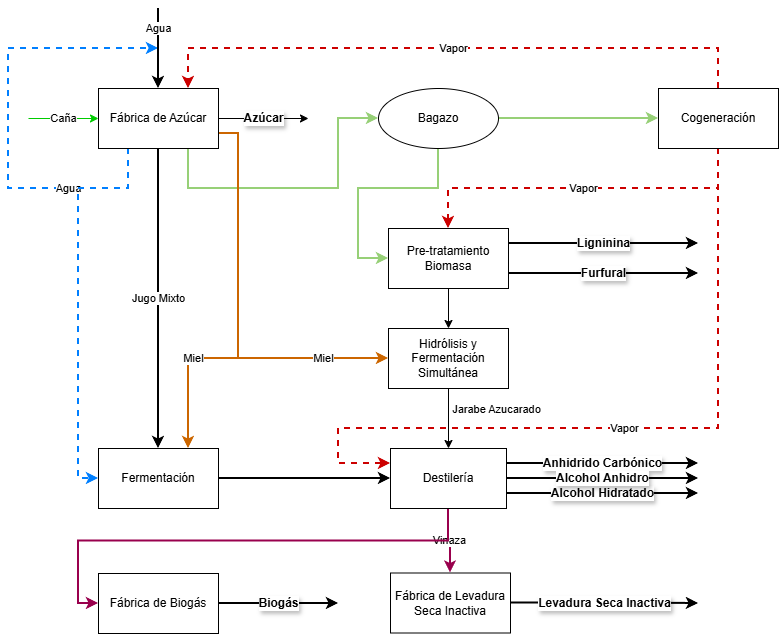
\includegraphics[width=1\linewidth,height=\textheight,keepaspectratio]{Esquema_Refineria.png}

}

\caption{\label{fig-arquitectura-biorrefineria}Arquitectura de
Valorización Integral en la Biorrefinería 4.0: Rutas de diversificación
y economía circular.}

\end{figure}%

\hfill\break

Bajo este paradigma, la \textbf{Biorrefinería 4.0} se aleja de la lógica
de optimización lineal de la factoría tradicional para transformarse en
un sistema de arbitraje multiproducto. La hibridación de algoritmos
permite que la planta no solo reaccione a las condiciones técnicas
\citep{davis2019}, sino que prepare su configuración operativa para
maximizar la rentabilidad marginal de cada flujo
\citep{mandegari2017, meramo-hurtado2020}. La diversificación efectiva,
por tanto, mide la madurez de la DMU para transformar el residuo en
recurso, reduciendo la vulnerabilidad del ingenio ante la volatilidad de
los precios internacionales mediante una canasta de outputs resiliente y
circular.\\

\begin{figure}[H]

\centering{

\pandocbounded{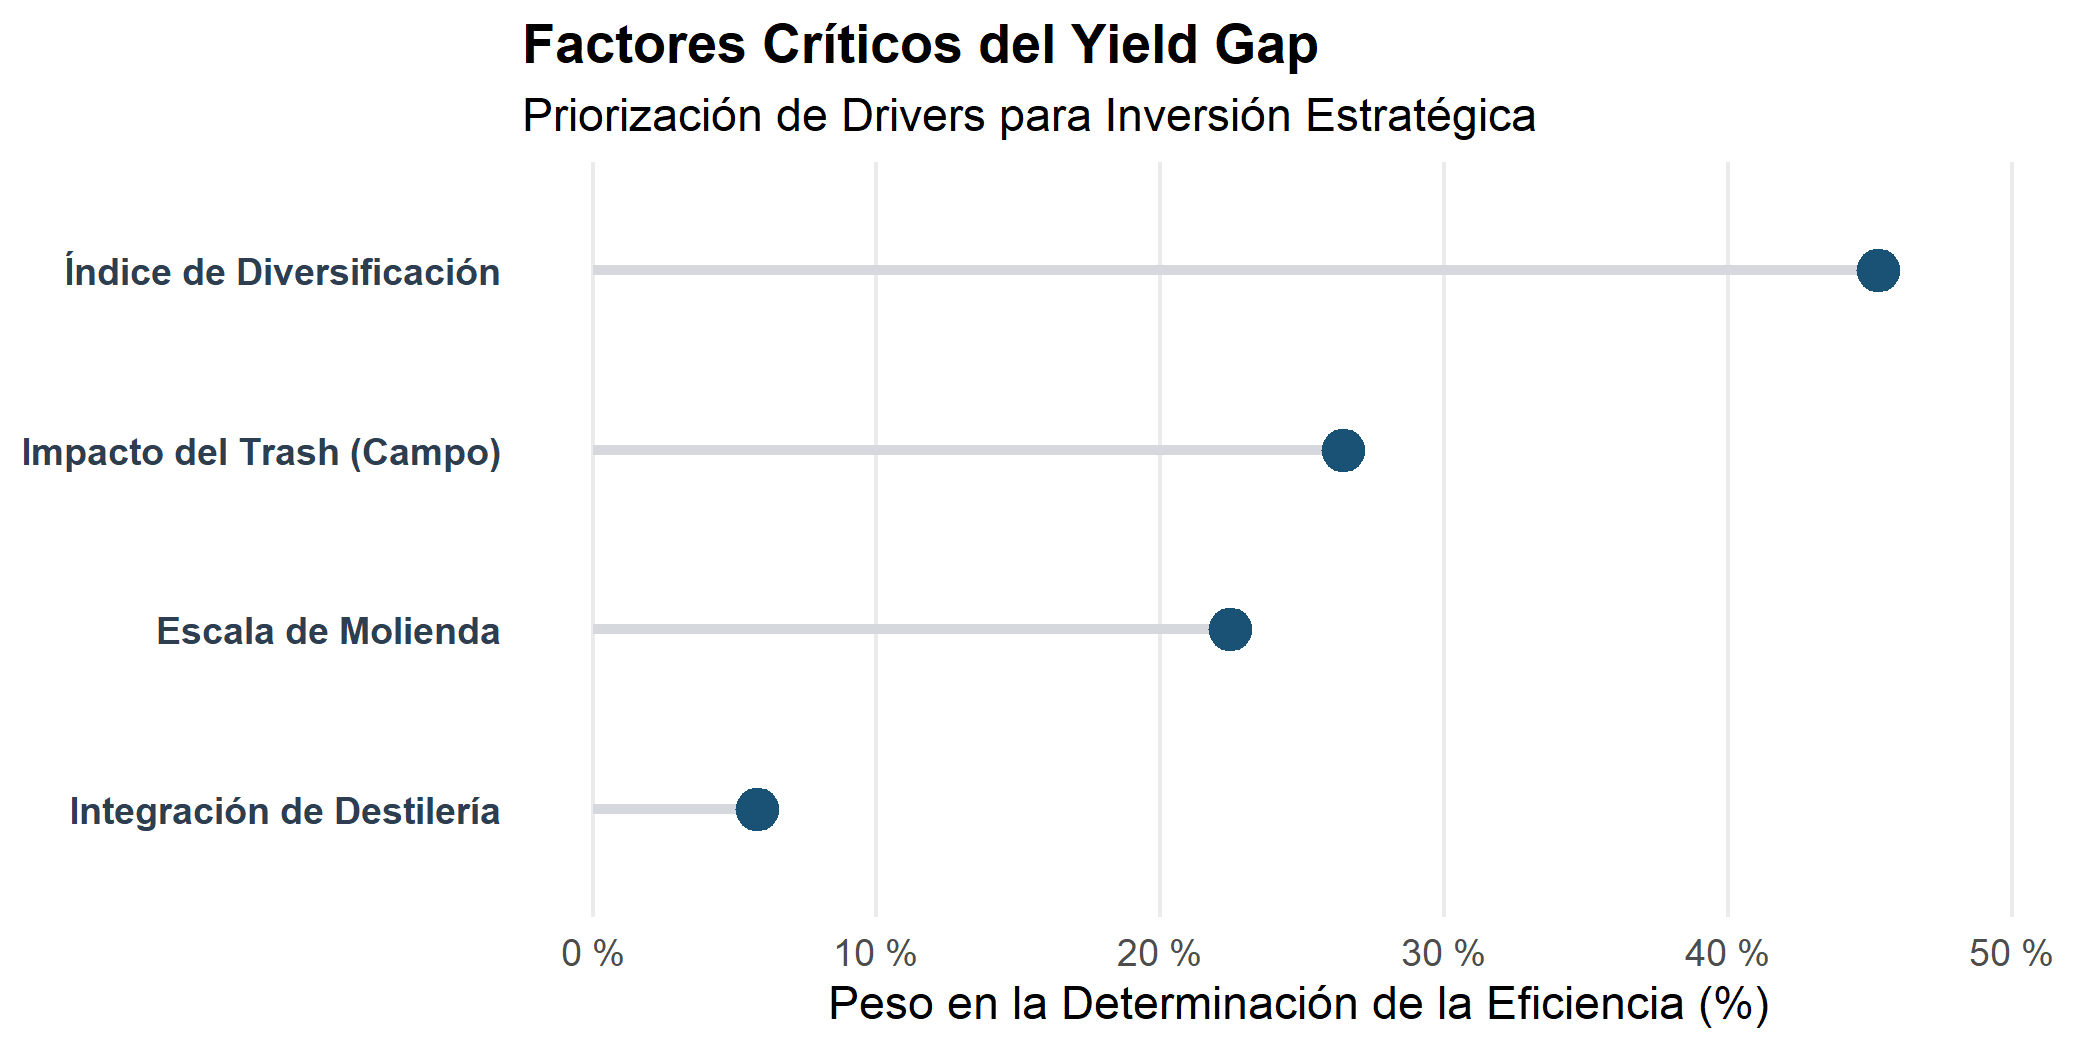
\includegraphics[keepaspectratio]{Ensayo_Biorrefineria_files/figure-pdf/fig-importancia-1.png}}

}

\caption{\label{fig-importancia}}

\end{figure}%

\hfill\break
La Figure~\ref{fig-importancia} revela la verdadera jerarquía de los
drivers de rentabilidad del sector, decodificados mediante algoritmos de
Random Forest. Los resultados arrojan una conclusión disruptiva para la
visión tradicional: el \textbf{Índice de Diversificación} se erige como
el determinante absoluto de la eficiencia técnica, confirmando que la
capacidad de arbitrar el \emph{product mix} (Biorrefinería 4.0) genera
un valor estratégico superior a la mera posesión de una destilería
física. Bajo este modelo, la destilería deja de ser un activo estático
para convertirse en una herramienta de agilidad comercial y estabilidad
técnica.

En segundo lugar, el análisis identifica al \textbf{Impacto del Trash}
como una fricción operativa que supera incluso a la Escala de Molienda
en su capacidad de destruir valor. Desde la perspectiva de la
inteligencia operativa, la materia extraña actúa como un
\textbf{``impuesto termodinámico''} que drena la capacidad de
evaporación y cristalización. Mientras que para un jefe de fábrica es
una variable exógena, para la gobernanza corporativa es una variable
endógena: los ingenios con fuerte integración vertical (como Ledesma)
logran blindar su frontera de eficiencia controlando la calidad desde el
surco, mientras que los seguidores ``importan'' la ineficiencia
logística de terceros.

Por lo tanto, cerrar el \emph{Yield Gap} en el NOA no es una cuestión de
comprar ``más fierros'' o aumentar el volumen de molienda (escala), sino
de \textbf{sofisticación analítica}. La inversión estratégica debe
migrar de los molinos hacia la digitalización prescriptiva de la cadena
de suministro agrícola. Solo mediante la integración de modelos que
gobiernen el flujo de biomasa desde el campo, los ingenios podrán
transformar su estructura de costos y alcanzar la resiliencia que define
a los líderes de la frontera eficiente.

\global\setlength{\Oldarrayrulewidth}{\arrayrulewidth}

\global\setlength{\Oldtabcolsep}{\tabcolsep}

\setlength{\tabcolsep}{2pt}

\renewcommand*{\arraystretch}{1.5}



\providecommand{\ascline}[3]{\noalign{\global\arrayrulewidth #1}\arrayrulecolor[HTML]{#2}\cline{#3}}

\begin{longtable}[c]{|p{1.20in}|p{1.30in}|p{3.50in}}

\caption{\label{tbl-jerarquia-drivers}Jerarquía de Impacto Estratégico:
Drivers de Eficiencia en el NOA}

\tabularnewline

\hhline{>{\arrayrulecolor[HTML]{666666}\global\arrayrulewidth=1.5pt}->{\arrayrulecolor[HTML]{666666}\global\arrayrulewidth=1.5pt}->{\arrayrulecolor[HTML]{666666}\global\arrayrulewidth=1.5pt}-}

\multicolumn{1}{>{\cellcolor[HTML]{1A5276}\raggedright}m{\dimexpr 1.2in+0\tabcolsep}}{\textcolor[HTML]{FFFFFF}{\fontsize{11}{11}\selectfont{\global\setmainfont{Arial}{\textbf{Driver\ Estratégico}}}}} & \multicolumn{1}{>{\cellcolor[HTML]{1A5276}\raggedright}m{\dimexpr 1.3in+0\tabcolsep}}{\textcolor[HTML]{FFFFFF}{\fontsize{11}{11}\selectfont{\global\setmainfont{Arial}{\textbf{Impacto\ en\ Eficiencia\ (θ)}}}}} & \multicolumn{1}{>{\cellcolor[HTML]{1A5276}\raggedright}m{\dimexpr 3.5in+0\tabcolsep}}{\textcolor[HTML]{FFFFFF}{\fontsize{11}{11}\selectfont{\global\setmainfont{Arial}{\textbf{Visión\ de\ Consultoría\ (CEO-Level)}}}}} \\

\noalign{\global\arrayrulewidth 0pt}\arrayrulecolor[HTML]{000000}

\hhline{>{\arrayrulecolor[HTML]{666666}\global\arrayrulewidth=1.5pt}->{\arrayrulecolor[HTML]{666666}\global\arrayrulewidth=1.5pt}->{\arrayrulecolor[HTML]{666666}\global\arrayrulewidth=1.5pt}-}\endfirsthead 

\hhline{>{\arrayrulecolor[HTML]{666666}\global\arrayrulewidth=1.5pt}->{\arrayrulecolor[HTML]{666666}\global\arrayrulewidth=1.5pt}->{\arrayrulecolor[HTML]{666666}\global\arrayrulewidth=1.5pt}-}

\multicolumn{1}{>{\cellcolor[HTML]{1A5276}\raggedright}m{\dimexpr 1.2in+0\tabcolsep}}{\textcolor[HTML]{FFFFFF}{\fontsize{11}{11}\selectfont{\global\setmainfont{Arial}{\textbf{Driver\ Estratégico}}}}} & \multicolumn{1}{>{\cellcolor[HTML]{1A5276}\raggedright}m{\dimexpr 1.3in+0\tabcolsep}}{\textcolor[HTML]{FFFFFF}{\fontsize{11}{11}\selectfont{\global\setmainfont{Arial}{\textbf{Impacto\ en\ Eficiencia\ (θ)}}}}} & \multicolumn{1}{>{\cellcolor[HTML]{1A5276}\raggedright}m{\dimexpr 3.5in+0\tabcolsep}}{\textcolor[HTML]{FFFFFF}{\fontsize{11}{11}\selectfont{\global\setmainfont{Arial}{\textbf{Visión\ de\ Consultoría\ (CEO-Level)}}}}} \\

\noalign{\global\arrayrulewidth 0pt}\arrayrulecolor[HTML]{000000}

\hhline{>{\arrayrulecolor[HTML]{666666}\global\arrayrulewidth=1.5pt}->{\arrayrulecolor[HTML]{666666}\global\arrayrulewidth=1.5pt}->{\arrayrulecolor[HTML]{666666}\global\arrayrulewidth=1.5pt}-}\endhead



\multicolumn{1}{>{\cellcolor[HTML]{E2EFDA}\raggedright}m{\dimexpr 1.2in+0\tabcolsep}}{\textcolor[HTML]{000000}{\fontsize{11}{11}\selectfont{\global\setmainfont{Arial}{\textbf{Diversificación}}}}} & \multicolumn{1}{>{\cellcolor[HTML]{E2EFDA}\raggedright}m{\dimexpr 1.3in+0\tabcolsep}}{\textcolor[HTML]{000000}{\fontsize{11}{11}\selectfont{\global\setmainfont{Arial}{\textbf{Máximo\ (Líder)}}}}} & \multicolumn{1}{>{\cellcolor[HTML]{E2EFDA}\raggedright}m{\dimexpr 3.5in+0\tabcolsep}}{\textcolor[HTML]{000000}{\fontsize{11}{11}\selectfont{\global\setmainfont{Arial}{No\ es\ 'tener\ una\ destilería',\ es\ la\ agilidad\ de\ arbitrar\ mercados\ y\ flujos\ de\ biomasa.}}}} \\

\noalign{\global\arrayrulewidth 0pt}\arrayrulecolor[HTML]{000000}

\hhline{>{\arrayrulecolor[HTML]{E5E5E5}\global\arrayrulewidth=1pt}->{\arrayrulecolor[HTML]{E5E5E5}\global\arrayrulewidth=1pt}->{\arrayrulecolor[HTML]{E5E5E5}\global\arrayrulewidth=1pt}-}



\multicolumn{1}{>{\raggedright}m{\dimexpr 1.2in+0\tabcolsep}}{\textcolor[HTML]{000000}{\fontsize{11}{11}\selectfont{\global\setmainfont{Arial}{Impacto\ Trash}}}} & \multicolumn{1}{>{\raggedright}m{\dimexpr 1.3in+0\tabcolsep}}{\textcolor[HTML]{000000}{\fontsize{11}{11}\selectfont{\global\setmainfont{Arial}{Crítico\ (Fricción)}}}} & \multicolumn{1}{>{\raggedright}m{\dimexpr 3.5in+0\tabcolsep}}{\textcolor[HTML]{000000}{\fontsize{11}{11}\selectfont{\global\setmainfont{Arial}{Impuesto\ logístico\ exógeno\ que\ destruye\ la\ capacidad\ térmica\ y\ fabril\ del\ ingenio.}}}} \\

\noalign{\global\arrayrulewidth 0pt}\arrayrulecolor[HTML]{000000}

\hhline{>{\arrayrulecolor[HTML]{E5E5E5}\global\arrayrulewidth=1pt}->{\arrayrulecolor[HTML]{E5E5E5}\global\arrayrulewidth=1pt}->{\arrayrulecolor[HTML]{E5E5E5}\global\arrayrulewidth=1pt}-}



\multicolumn{1}{>{\raggedright}m{\dimexpr 1.2in+0\tabcolsep}}{\textcolor[HTML]{000000}{\fontsize{11}{11}\selectfont{\global\setmainfont{Arial}{Escala\ (Molienda)}}}} & \multicolumn{1}{>{\raggedright}m{\dimexpr 1.3in+0\tabcolsep}}{\textcolor[HTML]{000000}{\fontsize{11}{11}\selectfont{\global\setmainfont{Arial}{Secundario}}}} & \multicolumn{1}{>{\raggedright}m{\dimexpr 3.5in+0\tabcolsep}}{\textcolor[HTML]{000000}{\fontsize{11}{11}\selectfont{\global\setmainfont{Arial}{El\ tamaño\ no\ garantiza\ eficiencia\ si\ la\ gestión\ sigue\ anclada\ en\ modelos\ analógicos.}}}} \\

\noalign{\global\arrayrulewidth 0pt}\arrayrulecolor[HTML]{000000}

\hhline{>{\arrayrulecolor[HTML]{E5E5E5}\global\arrayrulewidth=1pt}->{\arrayrulecolor[HTML]{E5E5E5}\global\arrayrulewidth=1pt}->{\arrayrulecolor[HTML]{E5E5E5}\global\arrayrulewidth=1pt}-}



\multicolumn{1}{>{\raggedright}m{\dimexpr 1.2in+0\tabcolsep}}{\textcolor[HTML]{000000}{\fontsize{11}{11}\selectfont{\global\setmainfont{Arial}{Integración\ Física}}}} & \multicolumn{1}{>{\raggedright}m{\dimexpr 1.3in+0\tabcolsep}}{\textcolor[HTML]{000000}{\fontsize{11}{11}\selectfont{\global\setmainfont{Arial}{Marginal}}}} & \multicolumn{1}{>{\raggedright}m{\dimexpr 3.5in+0\tabcolsep}}{\textcolor[HTML]{000000}{\fontsize{11}{11}\selectfont{\global\setmainfont{Arial}{El\ hardware\ sin\ inteligencia\ operativa\ (4.0)\ representa\ capital\ inmovilizado.}}}} \\

\noalign{\global\arrayrulewidth 0pt}\arrayrulecolor[HTML]{000000}

\hhline{>{\arrayrulecolor[HTML]{666666}\global\arrayrulewidth=1.5pt}->{\arrayrulecolor[HTML]{666666}\global\arrayrulewidth=1.5pt}->{\arrayrulecolor[HTML]{666666}\global\arrayrulewidth=1.5pt}-}


\end{longtable}

\arrayrulecolor[HTML]{000000}

\global\setlength{\arrayrulewidth}{\Oldarrayrulewidth}

\global\setlength{\tabcolsep}{\Oldtabcolsep}

\renewcommand*{\arraystretch}{1}

\begin{figure}[H]

\centering{

\pandocbounded{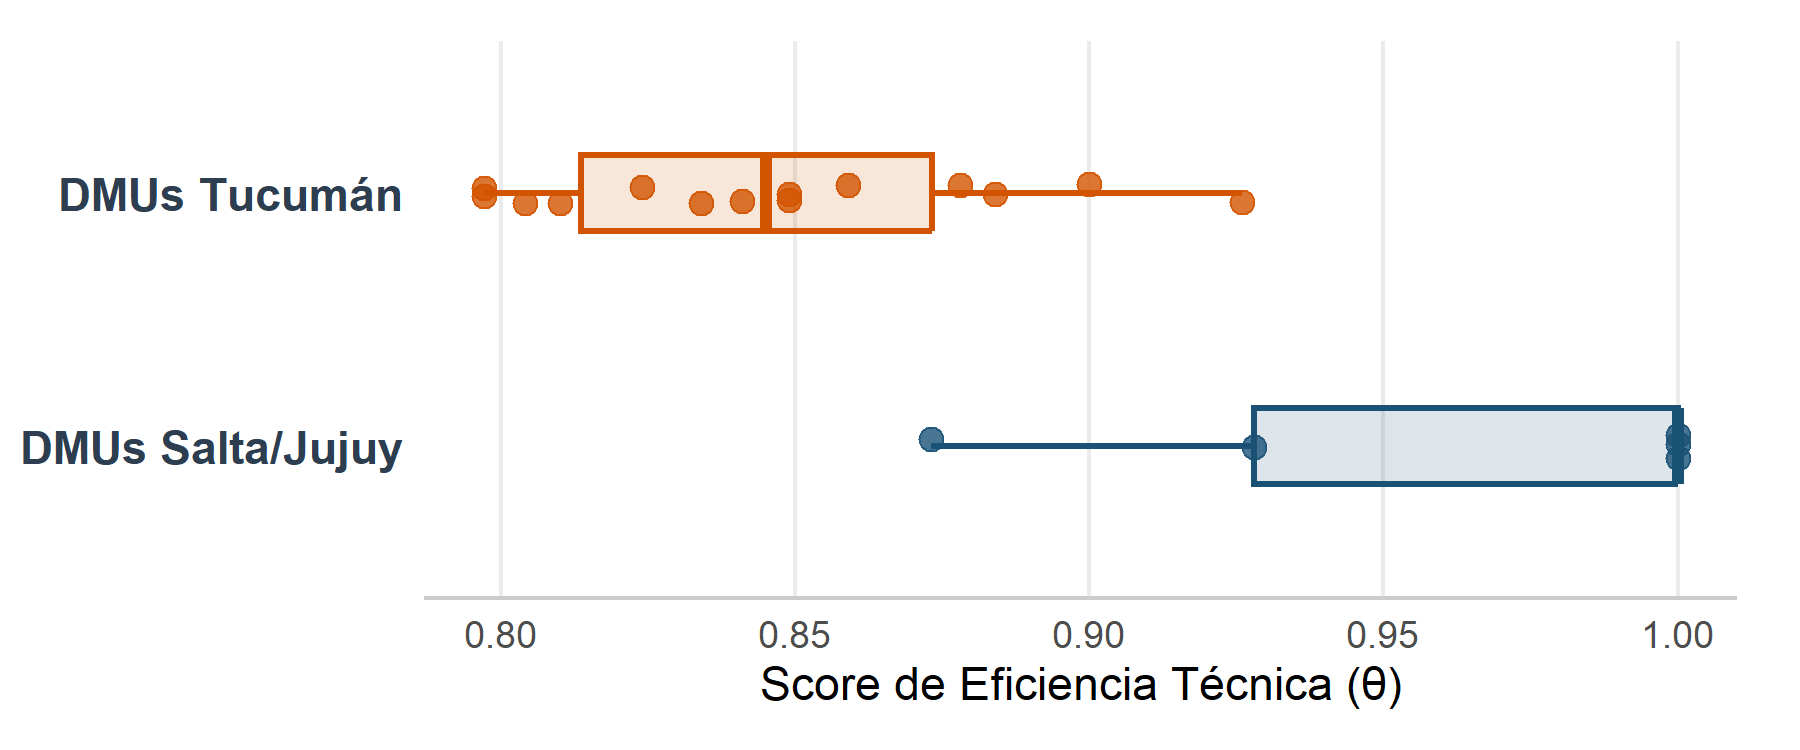
\includegraphics[keepaspectratio]{Ensayo_Biorrefineria_files/figure-pdf/fig-provincias-1.png}}

}

\caption{\label{fig-provincias}Distribución de la Eficiencia Técnica (θ)
por Grupos Provinciales (Zafra 2025).}

\end{figure}%

\hfill\break
Como se detalla en la Figure~\ref{fig-provincias}, la eficiencia técnica
regional presenta una asimetría estructural. Las DMUs de Salta y Jujuy
operan con una mediana de \(\theta\) marcadamente superior y una menor
volatilidad operativa en comparación con las de Tucumán. Esta
resiliencia de la frontera norte se fundamenta en un modelo de doble
apalancamiento: por un lado, la \textbf{Diversificación} extrema
(variable líder en la Figure~\ref{fig-importancia}) que utiliza la
destilería como un estabilizador económico y térmico; y por el otro, una
fuerte \textbf{integración vertical hacia atrás}.

A diferencia de la fragmentación de la propiedad de la tierra en
Tucumán, el modelo de gestión agrícola centralizada en el Norte permite
a estos ingenios gobernar su cadena de suministro. Al controlar la
cosecha, estas DMUs logran mitigar drásticamente el \textbf{Impacto del
Trash} desde el surco. Esta gobernanza transforma una variable exógena e
incontrolable para los tucumanos en un parámetro endógeno y optimizado,
asegurando que el tren de molienda procese biomasa limpia y blindando el
balance termodinámico del complejo.

En consecuencia, esta `autopsia técnica' confirma que el rezago en los
ingenios seguidores es el resultado de una doble vulnerabilidad: el
confinamiento en modelos de producto único (baja diversificación) y la
exposición crónica a ineficiencias importadas del campo (alto trash). La
analítica avanzada concluye que cerrar el \emph{Yield Gap} regional
requiere abandonar la gestión reactiva y trascender la inversión
exclusiva en `fierros' fabriles (escala física).

El salto hacia la frontera exige orientar el CAPEX mediante una visión
sistémica: financiar la diversificación inteligente de la matriz de
productos e integrar digitalmente la logística de cosecha. Reducir la
carga cognitiva gerencial implica desplegar modelos prescriptivos que
detecten automatizadamente las pérdidas invisibles, desde la fricción en
el cañaveral hasta las fugas en el balance térmico, emulando así la
agilidad estratégica de los líderes de la región.

\section{El Rol de la Auditoría Técnica y la Madurez
Digital}\label{el-rol-de-la-auditoruxeda-tuxe9cnica-y-la-madurez-digital}

Desde una perspectiva de \textbf{consultoría estratégica}, la
ineficiencia en el NOA no es un problema de voluntad técnica, sino de
\textbf{arquitectura de información y gobernanza de datos}. Los
registros del IPAAT, aunque valiosos, actúan hoy como un ``retrovisor''
histórico y no como un sistema de navegación en tiempo real. Como
académicos, debemos señalar que esta ``ceguera operativa'' ---la
incapacidad de cuantificar las pérdidas invisibles en el balance térmico
o de anticipar el impacto exógeno del trash de caña sobre la molienda---
es lo que mantiene a los ``Ingenios Seguidores'' anclados debajo de la
frontera de eficiencia \citep{zhu2022}. La auditoría técnica basada en
la hibridación DEA-ML permite una \textbf{transparencia radical:} el
índice \(\theta\) deja de ser una mera percepción fabril para
convertirse en un indicador objetivo del \emph{Yield Gap} sistémico.
Como sostiene \citep{zhu2022}, el uso de DEA en entornos de datos
complejos audita la veracidad de los reportes industriales; pero al
integrarlo con algoritmos predictivos, transformamos esos registros
históricos en modelos de analítica prescriptiva que expanden el control
gerencial desde el surco hasta la destilería.

\section{Conclusiones y Roadmap: Hacia el Modelo de
Optimización}\label{conclusiones-y-roadmap-hacia-el-modelo-de-optimizaciuxf3n}

El tránsito hacia la Biorrefinería 4.0 en el NOA no es un desafío de
adquisición de bienes de capital, sino de arquitectura de decisión. La
evidencia de este ensayo demuestra que el simple emplazamiento de una
destilería posee un poder explicativo marginal sobre el éxito operativo.
La verdadera hoja de ruta hacia la frontera técnica se sintetiza en tres
pilares estratégicos:

\begin{enumerate}
\def\labelenumi{\arabic{enumi}.}
\item
  \textbf{De la ``Autopsia'' a la Prospección Sistémica
  (Campo-Fábrica):} Si bien el uso de \textbf{Machine Learning (Random
  Forest)} permite realizar ``autopsias'' precisas sobre la ineficiencia
  histórica, el imperativo de la Biorrefinería 4.0 es institucionalizar
  estos modelos como herramientas de prospección integral. No basta con
  identificar \emph{ex-post} que la inestabilidad en el caudal de vapor
  o el exceso de trash destruyeron el score de eficiencia \(\theta\). La
  verdadera ventaja radica en la hibridación DEA-ML para anticipar el
  impacto de variables exógenas logísticas y transformarlas en
  \textbf{oportunidades de arbitraje}. Esto permite al gestor proyectar
  la configuración operativa óptima en tiempo real, desde el control de
  calidad en el surco hasta el \emph{mix} de productos
  (azúcar/bioetanol) dictado por el mercado.
\item
  \textbf{Reducción de la Carga Cognitiva y Madurez Digital:} El CEO no
  requiere más registros históricos o tablas de Excel que actúan como
  ``retrovisores'' operativos. La propuesta de hibridación DEA-ML actúa
  como un filtro de \textbf{Inteligencia Operativa} que traduce la
  complejidad técnica en un \textbf{Tablero de Optimización Sistémica}.
  Al automatizar la detección de desviaciones y entregar conclusiones
  prescriptivas, se reduce la carga cognitiva gerencial, permitiendo que
  la dirección se enfoque en la arquitectura de información y en la
  agilidad organizacional necesaria para responder a los datos.
\item
  \textbf{El Salto Tecnológico como Opción Financiera Física:} La
  evidencia es concluyente: los ingenios diversificados y con
  integración vertical (como los líderes de Salta/Jujuy) no solo son más
  eficientes, sino más resilientes. Bajo el paradigma 4.0, la inversión
  en una destilería no debe verse solo como infraestructura, sino como
  una \textbf{``opción financiera física''} que otorga la flexibilidad
  necesaria para estabilizar la rentabilidad ante la volatilidad de
  precios y la fricción de la materia prima. La capacidad de gobernar la
  cadena de suministro y transformar el residuo en recurso es la medida
  definitiva de la madurez de una DMU para liderar la bioeconomía
  regional.
\end{enumerate}

\global\setlength{\Oldarrayrulewidth}{\arrayrulewidth}

\global\setlength{\Oldtabcolsep}{\tabcolsep}

\setlength{\tabcolsep}{2pt}

\renewcommand*{\arraystretch}{1.5}



\providecommand{\ascline}[3]{\noalign{\global\arrayrulewidth #1}\arrayrulecolor[HTML]{#2}\cline{#3}}

\begin{longtable}[c]{|p{1.40in}|p{2.20in}|p{2.60in}}

\caption{\label{tbl-comparativa-paradigmas}Síntesis Estratégica: Del
Paradigma Tradicional a la Biorrefinería 4.0}

\tabularnewline

\hhline{>{\arrayrulecolor[HTML]{666666}\global\arrayrulewidth=1.5pt}->{\arrayrulecolor[HTML]{666666}\global\arrayrulewidth=1.5pt}->{\arrayrulecolor[HTML]{666666}\global\arrayrulewidth=1.5pt}-}

\multicolumn{1}{>{\centering}m{\dimexpr 1.4in+0\tabcolsep}}{\textcolor[HTML]{000000}{\fontsize{11}{11}\selectfont{\global\setmainfont{Arial}{\textbf{Dimensión\ Analítica}}}}} & \multicolumn{1}{>{\centering}m{\dimexpr 2.2in+0\tabcolsep}}{\textcolor[HTML]{000000}{\fontsize{11}{11}\selectfont{\global\setmainfont{Arial}{\textbf{Paradigma\ Tradicional}}}}\textcolor[HTML]{000000}{\fontsize{11}{11}\selectfont{\global\setmainfont{Arial}{\textbf{\linebreak }}}}\textcolor[HTML]{000000}{\fontsize{11}{11}\selectfont{\global\setmainfont{Arial}{\textbf{(Seguidores\ NOA)}}}}} & \multicolumn{1}{>{\cellcolor[HTML]{C6E0B4}\centering}m{\dimexpr 2.6in+0\tabcolsep}}{\textcolor[HTML]{000000}{\fontsize{11}{11}\selectfont{\global\setmainfont{Arial}{\textbf{Biorrefinería\ Inteligente}}}}\textcolor[HTML]{000000}{\fontsize{11}{11}\selectfont{\global\setmainfont{Arial}{\textbf{\linebreak }}}}\textcolor[HTML]{000000}{\fontsize{11}{11}\selectfont{\global\setmainfont{Arial}{\textbf{(Frontera\ DEA-ML)}}}}} \\

\noalign{\global\arrayrulewidth 0pt}\arrayrulecolor[HTML]{000000}

\hhline{>{\arrayrulecolor[HTML]{666666}\global\arrayrulewidth=1.5pt}->{\arrayrulecolor[HTML]{666666}\global\arrayrulewidth=1.5pt}->{\arrayrulecolor[HTML]{666666}\global\arrayrulewidth=1.5pt}-}\endfirsthead 

\hhline{>{\arrayrulecolor[HTML]{666666}\global\arrayrulewidth=1.5pt}->{\arrayrulecolor[HTML]{666666}\global\arrayrulewidth=1.5pt}->{\arrayrulecolor[HTML]{666666}\global\arrayrulewidth=1.5pt}-}

\multicolumn{1}{>{\centering}m{\dimexpr 1.4in+0\tabcolsep}}{\textcolor[HTML]{000000}{\fontsize{11}{11}\selectfont{\global\setmainfont{Arial}{\textbf{Dimensión\ Analítica}}}}} & \multicolumn{1}{>{\centering}m{\dimexpr 2.2in+0\tabcolsep}}{\textcolor[HTML]{000000}{\fontsize{11}{11}\selectfont{\global\setmainfont{Arial}{\textbf{Paradigma\ Tradicional}}}}\textcolor[HTML]{000000}{\fontsize{11}{11}\selectfont{\global\setmainfont{Arial}{\textbf{\linebreak }}}}\textcolor[HTML]{000000}{\fontsize{11}{11}\selectfont{\global\setmainfont{Arial}{\textbf{(Seguidores\ NOA)}}}}} & \multicolumn{1}{>{\cellcolor[HTML]{C6E0B4}\centering}m{\dimexpr 2.6in+0\tabcolsep}}{\textcolor[HTML]{000000}{\fontsize{11}{11}\selectfont{\global\setmainfont{Arial}{\textbf{Biorrefinería\ Inteligente}}}}\textcolor[HTML]{000000}{\fontsize{11}{11}\selectfont{\global\setmainfont{Arial}{\textbf{\linebreak }}}}\textcolor[HTML]{000000}{\fontsize{11}{11}\selectfont{\global\setmainfont{Arial}{\textbf{(Frontera\ DEA-ML)}}}}} \\

\noalign{\global\arrayrulewidth 0pt}\arrayrulecolor[HTML]{000000}

\hhline{>{\arrayrulecolor[HTML]{666666}\global\arrayrulewidth=1.5pt}->{\arrayrulecolor[HTML]{666666}\global\arrayrulewidth=1.5pt}->{\arrayrulecolor[HTML]{666666}\global\arrayrulewidth=1.5pt}-}\endhead



\multicolumn{1}{>{\raggedright}m{\dimexpr 1.4in+0\tabcolsep}}{\textcolor[HTML]{000000}{\fontsize{11}{11}\selectfont{\global\setmainfont{Arial}{\textbf{Rol\ de\ los\ Datos}}}}} & \multicolumn{1}{>{\raggedright}m{\dimexpr 2.2in+0\tabcolsep}}{\textcolor[HTML]{000000}{\fontsize{11}{11}\selectfont{\global\setmainfont{Arial}{Registro\ histórico\ y\ descriptivo\ (Excel).}}}} & \multicolumn{1}{>{\cellcolor[HTML]{E2EFDA}\raggedright}m{\dimexpr 2.6in+0\tabcolsep}}{\textcolor[HTML]{000000}{\fontsize{11}{11}\selectfont{\global\setmainfont{Arial}{Activo\ prescriptivo\ y\ de\ arbitraje\ en\ tiempo\ real.}}}} \\

\noalign{\global\arrayrulewidth 0pt}\arrayrulecolor[HTML]{000000}

\hhline{>{\arrayrulecolor[HTML]{666666}\global\arrayrulewidth=0.75pt}->{\arrayrulecolor[HTML]{666666}\global\arrayrulewidth=0.75pt}->{\arrayrulecolor[HTML]{666666}\global\arrayrulewidth=0.75pt}-}



\multicolumn{1}{>{\raggedright}m{\dimexpr 1.4in+0\tabcolsep}}{\textcolor[HTML]{000000}{\fontsize{11}{11}\selectfont{\global\setmainfont{Arial}{\textbf{Gestión\ de\ Eficiencia}}}}} & \multicolumn{1}{>{\raggedright}m{\dimexpr 2.2in+0\tabcolsep}}{\textcolor[HTML]{000000}{\fontsize{11}{11}\selectfont{\global\setmainfont{Arial}{Reactiva\ (Mantenimiento\ físico\ y\ 'fierros').}}}} & \multicolumn{1}{>{\cellcolor[HTML]{E2EFDA}\raggedright}m{\dimexpr 2.6in+0\tabcolsep}}{\textcolor[HTML]{000000}{\fontsize{11}{11}\selectfont{\global\setmainfont{Arial}{Proactiva\ (Algoritmos\ orientados\ a\ outputs).}}}} \\

\noalign{\global\arrayrulewidth 0pt}\arrayrulecolor[HTML]{000000}

\hhline{>{\arrayrulecolor[HTML]{666666}\global\arrayrulewidth=0.75pt}->{\arrayrulecolor[HTML]{666666}\global\arrayrulewidth=0.75pt}->{\arrayrulecolor[HTML]{666666}\global\arrayrulewidth=0.75pt}-}



\multicolumn{1}{>{\raggedright}m{\dimexpr 1.4in+0\tabcolsep}}{\textcolor[HTML]{000000}{\fontsize{11}{11}\selectfont{\global\setmainfont{Arial}{\textbf{Tratamiento\ del\ Trash}}}}} & \multicolumn{1}{>{\raggedright}m{\dimexpr 2.2in+0\tabcolsep}}{\textcolor[HTML]{000000}{\fontsize{11}{11}\selectfont{\global\setmainfont{Arial}{Gasto\ logístico\ inevitable\ (Variable\ exógena\ ignorada).}}}} & \multicolumn{1}{>{\cellcolor[HTML]{E2EFDA}\raggedright}m{\dimexpr 2.6in+0\tabcolsep}}{\textcolor[HTML]{000000}{\fontsize{11}{11}\selectfont{\global\setmainfont{Arial}{Impuesto\ termodinámico\ a\ minimizar\ (Frontera\ de\ Fricción).}}}} \\

\noalign{\global\arrayrulewidth 0pt}\arrayrulecolor[HTML]{000000}

\hhline{>{\arrayrulecolor[HTML]{666666}\global\arrayrulewidth=0.75pt}->{\arrayrulecolor[HTML]{666666}\global\arrayrulewidth=0.75pt}->{\arrayrulecolor[HTML]{666666}\global\arrayrulewidth=0.75pt}-}



\multicolumn{1}{>{\raggedright}m{\dimexpr 1.4in+0\tabcolsep}}{\textcolor[HTML]{000000}{\fontsize{11}{11}\selectfont{\global\setmainfont{Arial}{\textbf{Toma\ de\ Decisiones}}}}} & \multicolumn{1}{>{\raggedright}m{\dimexpr 2.2in+0\tabcolsep}}{\textcolor[HTML]{000000}{\fontsize{11}{11}\selectfont{\global\setmainfont{Arial}{Alta\ carga\ cognitiva\ por\ silos\ de\ información.}}}} & \multicolumn{1}{>{\cellcolor[HTML]{E2EFDA}\raggedright}m{\dimexpr 2.6in+0\tabcolsep}}{\textcolor[HTML]{000000}{\fontsize{11}{11}\selectfont{\global\setmainfont{Arial}{Inteligencia\ Operativa\ centralizada\ (Modelos\ Híbridos).}}}} \\

\noalign{\global\arrayrulewidth 0pt}\arrayrulecolor[HTML]{000000}

\hhline{>{\arrayrulecolor[HTML]{666666}\global\arrayrulewidth=1.5pt}->{\arrayrulecolor[HTML]{666666}\global\arrayrulewidth=1.5pt}->{\arrayrulecolor[HTML]{666666}\global\arrayrulewidth=1.5pt}-}


\end{longtable}

\arrayrulecolor[HTML]{000000}

\global\setlength{\arrayrulewidth}{\Oldarrayrulewidth}

\global\setlength{\tabcolsep}{\Oldtabcolsep}

\renewcommand*{\arraystretch}{1}

\textbf{Conclusión Final:} El modelo de optimización propuesto no es una
mejora incremental; es una ruptura de paradigma. Para cerrar el
\emph{Yield Gap} regional, el NOA debe cruzar el abismo que separa la
intuición analógica de la prospección digital. La hibridación DEA-ML
transforma cada ingenio en un \textbf{nodo inteligente} capaz de
arbitrar con precisión matemática su destino productivo, reduciendo la
complejidad sistémica a conclusiones estratégicas accionables. El futuro
de la biorrefinería en Argentina no se escribirá en planillas de
cálculo, sino en la capacidad de procesar la incertidumbre mediante la
soberanía analítica.

\newpage


\renewcommand\refname{Bibliografia}
\bibliography{bibliografia.bib}



\end{document}
